% vim: set spelllang=fr foldmethod=marker:
\chapter{Sélection aléatoire des \cns}

% préfixe: sa
\renewcommand\chapterpath{Main/SelecAleatoire}
\renewcommand\chapterfig{Main/SelecAleatoire/Figures}

Dernière édition: \today
%\usepackage{amsmath}
%\usepackage{booktabs}
%\usepackage{float}
%\usepackage{flushend}
%\usepackage{setspace}
%\usepackage{subfigure}
%\usepackage{wrapfig}
%\newcommand\apriori{\textit{a priori}\xspace}
%\newcommand\aposteriori{\textit{a posteriori}\xspace}
%\newcommand\defacto{\textit{de facto}\xspace}
%\newcommand\eg{\textit{e.~g.}\xspace}
%\newcommand\via{\textit{via}\xspace}
%\newcommand\etc{\textit{et cætera}\xspace}
%\newcommand\BS{\textit{BS}\xspace}
%\newcommand\ch{\textit{cluster head}\xspace}
%\newcommand\chs{\textit{cluster heads}\xspace}
%\newcommand\CH{\textit{CH}\xspace}
%\newcommand\leach{\textit{LEACH}\xspace}
%\newcommand\cn{\textit{cNode}\xspace}
%\newcommand\cns{\textit{cNodes}\xspace}
%\newcommand\ns{\textsf{ns-2}\xspace}
%\newcommand\todo[1]{\textcolor{red}{\textbf{TODO: }#1}}

\paragraph{abstract}
Ce document est un travail de synthèse reprenant les éléments présentés dans l'article \textit{Modeling tools for detecting DoS attacks in WSNs}~\cite{BMM13}.
Il constitue une base en vue de l'insertion en tant que chapitre dans le mémoire de thèse de l'auteur.\\

L'article en question exposait une solution dynamique permettant la détection de nœuds compromis dans les réseaux de capteurs sans fils (WSN).
En outre, il mettait en avant des résultats obtenus à partir de simulations réalisées sur le logiciel \ns, ainsi que la modélisation du système sous forme de chaînes de Markov et de réseaux de Petri.\\

Ce document se décompose comme suit:
\begin{itemize}
	\item en section~\ref{sa:sec:contexte} est introduit le contexte des travaux présentés: y sont présentés les réseaux de capteurs sans fil, ainsi que des mécanismes relatifs à la partition de ce réseau en plusieurs clusters;
	\item la section~\ref{sa:sec:detection} développe la méthode proposée dans l'article associé~\cite{BMM13}, destinée à détecter certaines attaques de type «~déni de service~» dans ces réseaux de capteurs sans fil. Serons notamment traitées les problématiques d'élection statique ou, au contraire, dynamique des nœuds de contrôle chargés de monitorer le trafic;
	\item une fois la méthode exposée, nous présenterons en section~\ref{sa:sec:modelisation} plusieurs modèles de cette solution: sous forme de chaînes de Markov tout d'abord, puis sous forme de réseaux de Petri stochastiques généralisés étendus, avant de rajouter une surcouche en logique stochastique avec automates hybrides;
	\item enfin, la section~\ref{sa:sec:resultats} fera état des valeurs numériques obtenues en simulant la solution à l'aide de l'outil \ns.
\end{itemize}

% vim: set spelllang=fr foldmethod=marker:
\section{Contexte}
\label{sa:sec:contexte}
%===============================================================================
    \subsection{Réseaux de capteurs sans fil}

        \subsubsection{De quoi s'agit-il?}
Les réseaux de capteurs sans fil, ou \textit{WSN} (pour \textit{Wireless Sensor Networks} en anglais), sont des réseaux constitués de petits appareils, les capteurs, ainsi que d'une station de base.
Les capteurs échangent par communications hertziennes, en utilisant des protocoles tels IEEE~802.11.
Le routage des paquets dans le réseau peut faire appel à l'un des nombreux protocoles développés à cet effet (par exemple: \textit{AODV}, \textit{OLSR}), qu'il repose sur un algorithme centralisé (dirigé par une seule entité) ou distribué (exécuté par chaque entité du réseau).
Ils collectent des informations sur leur environnement et les font remonter à la station de base.
Cette station de base, ou \BS (pour \textit{Base Station}), parfois appelée \textit{puits} (ou \textit{sink} en anglais), est chargée de récolter et traiter les données provenant des capteurs.
Une fois les capteurs déployés, l'administrateur n'interagit plus avec le réseau que par le biais de la station de base.

Quel que soit le protocole de liaison de données utilisé, il est rare que tous les capteurs d'un WSN soit directement connectés les uns aux autres.
À la topologie d'un réseau donné est donc très souvent associé le graphe de connectivité du réseau.
Pour cette raison, dans la littérature comme dans la suite de ce document, il sera souvent fait référence aux capteurs sous le terme de \textit{nœuds} (\textit{nodes} en anglais).

        \subsubsection{Applications}
Le champ d'application des WSN est très vaste.
Des réseaux peuvent être mis en place en forêt, par exemple, afin de détecter les départs de feu et de lutter plus efficacement contre les incendies.
D'autres peuvent être déployés en mer, afin de mesurer le taux de pollution des eaux.
En zones à risques, les capteurs peuvent être utilisés pour mesurer l'activité sismique ou volcanique du sol, et permettre une meilleure anticipation des phénomènes naturels.

Les WSN sont également utilisés dans certains milieux critiques.
Un exemple serait leur usage dans le domaine du nucléaire.
Un autre, de taille, est leur exploitation intensive par les militaires sur les champs de batailles, afin de relier fantassins et véhicules de tous types; un maximum d'informations doit alors être remonté au centre de commandement, afin de permettre une supervision optimale des forces en mouvement.

Un autre domaine d'application en voie de développement est ce que l'on appelle l'\textit{Internet des objets} (\textit{the Internet of things} en anglais), et qui consiste en quelque sorte à étendre Internet au monde réel, par le biais d'une interconnexion réseau entre les objets de la vie courante.

        \subsubsection{Contraintes en ressources}
De par leur petite taille, et à cause de leurs déploiement dans des zones souvent difficiles d'accès, les capteurs n'embarquent qu'une quantité limitée de matériel, qui ne peut pas toujours être remplacé.
Les capteurs se retrouvent donc avec des capacités limitées, notamment en ce qui concerne:
\begin{itemize}
    \item les capacités de calcul: les processeurs embarqués sont relativement peu puissants.
        Les algorithmes exécutés par les capteurs doivent donc être de complexité relativement basse;
    \item les capacités de mémoire: les capteurs disposent de RAM et d'un peu d'espace de stockage, mais ils ne sont pas du tout conçus pour sauvegarder de grandes bases de données.
        Les informations récoltées doivent être acheminées à la station de base, et non stockées sur le long terme par les capteurs eux-mêmes;
    \item l'énergie disponible: les capteurs disposent d'une batterie qui leur fournit une quantité d'énergie finie, et (la plupart du temps) non rechargeable.
        Il est donc essentiel de conserver à l'esprit une gestion parcimonieuse de l'énergie pour tout programme implémenté sur les capteurs.
        Des calculs importants, ainsi que des émissions/réceptions d'ondes électromagnétiques nombreuses ou mal gérées, sont les principaux facteurs d'un épuisement prématuré de la batterie. 
\end{itemize}

Il est à noter qu'au regard de ces contraintes qui affectent les capteurs, la station de base est considérée comme disposant de capacités illimitées.

        \subsubsection{Sécurité}
En raison de leurs faibles capacités, conjuguées aux domaines critiques dans lesquels ils interviennent parfois, les capteurs peuvent présenter des cibles de choix pour un attaquant.
Les algorithmes et mécanismes classiques utilisés en cryptographie afin d'assurer la confidentialité ou l'authentification des données sont souvent très exigeants en ressources (en termes de calcul notamment, et donc de consommation énergétique).
Il a fallu adapter ces mécanismes aux capteurs.

D'autres attaques peuvent être menées, non plus pour intercepter des données, mais dans le but de perturber le bon fonctionnement du réseau.
Ce sont les attaques dites de \textit{déni de service}.
Un attaquant, par le biais d'un nœud compromis par exemple, peut ainsi chercher à détourner des flux de données au sein du réseau, à empêcher des paquets de parvenir à destination (en les supprimant), à maximiser le débit du nœud compromis au détriment de celui des autres nœuds, à saturer le canal pour empêcher les nœuds légitimes de l'utiliser, ou encore à pousser les autres capteurs à l'épuisement de leurs réserves en énergie, \etc.

Notre but est ici de proposer, modéliser et tester une solution permettant de détecter, puis de réagir à une attaque de ce type, tout en assurant une consommation minimale en ressources pour les capteurs du réseau.
L'une des possibilités permettant de réduire la consommation en énergie est l'utilisation d'un réseau hiérarchiquement clusterisé.

%===============================================================================
    \subsection{Partition hiérarchique des nœuds du réseau}
    \label{sa:subsec:Partition}

        \subsubsection{Partition du réseau}
«~Clusteriser~» un ensemble d'éléments revient à le diviser en sous-ensembles appelés \textit{clusters}.
Dans le cas des réseaux de capteurs sans fil, cette partition permet d'obtenir un routage efficace des paquets, en adoptant la configuration suivante:
\begin{enumerate}
    \item tous les nœuds réunis au sein d'un même cluster sont capables de communiquer directement entre eux (\textit{one-hop transmission});
    \item lors de la partition, un unique nœud par cluster est désigné «~chef~» du cluster.
        Il est choisi, de façon déterministe ou bien aléatoire selon l'algorithme employé, parmi les nœuds «~normaux~» du cluster.
        Ce «~chef~» est appelé \ch (\CH);
    \item lorsqu'un capteur quelconque d'un cluster souhaite faire parvenir des informations à un nœud d'un autre cluster\footnote{Pour une grande partie des applications, les communications entre nœuds de différents clusters, hors \chs, ne se produisent pas. La totalité du trafic «~utile~», acheminant des données, est généralement à destination de la station de base.}, ou bien à la station de base, il envoie ses paquets de données au \ch de son cluster ;
    \item le \ch transmet alors les paquets de données, soit directement à la cible s'il s'agit de la station de base et qu'il peut l'atteindre, soit en passant par d'autres \chs (\textit{multi-hops transmission}), jusqu'à atteindre le destinataire.
\end{enumerate}
L'appel à un algorithme de clusterisation a pour effet de limiter les émissions à «~longue portée~» (relativement aux communications intra-clusters) aux \textit{cluster heads} seulement.
Hors les communications sur de plus grandes distances se traduisent par une plus grande consommation en énergie (puisqu'une plus grande puissance d'émission est nécessaire).
Les capteurs «~normaux~» (non \chs) n'ont pas à atteindre directement des nœuds situés en dehors de leur cluster; ils économisent d'autant en énergie.
De plus, dans la limite de leurs capacités, les \chs sont généralement amenés à réaliser des opérations d'agrégation voire parfois de compression sur les paquets qu'ils reçoivent, afin de limiter encore les transmissions coûteuses.

De nombreux algorithmes de clusterisation de données existent.
Plusieurs d'entre eux sont même spécifiquement adaptés aux réseaux de capteurs sans fil.
Parmi les plus fréquemment utilisés, on trouve des algorithmes comme \leach~\cite{HCB00} ou \textit{HEED}~\cite{YF04}.
D'autres sont moins connus, comme \textit{FFUCA}~\cite{FL11}, qui repose sur l'exploitation de propriétés ultramétriques dans le réseau.

        \subsubsection{Clusterisation hiérarchique}
Une fois le réseau de capteurs divisé en clusters, rien n'empêche de considérer les clusters un à un et de leur appliquer à nouveau un algorithme de clusterisation, de façon à établir des sous-ensembles dans chaque cluster.
Et ainsi de suite, de façon récursive, jusqu'à atteindre le degré de hiérarchie désiré.
L'intérêt de cette méthode est de créer une partition hiérarchique dans le réseau, permettant un meilleur contrôle des sous-ensembles de capteurs.
Par ailleurs, les clusters situés tout en bas dans la hiérarchie constituée seront de petite taille.
Les communications intra-clusters seront donc peu consommatrices en énergie.

Pour pouvoir distinguer plus facilement le niveau de hiérarchie auquel nous nous plaçons, nous désignerons par la suite sous le terme \textit{$k$-cluster} ($0 \leq k \leq$~nombre de capteurs) un sous-ensemble obtenu après $k$ applications de l'algorithme de clusterisation.
En suivant cette convention, l'unique $0$-cluster est alors le réseau tout entier.
Lorsque nous parlons simplement de \textit{clusters}, il faudra comprendre \textit{$1$-clusters}; autrement dit, des clusters issus d'une partition simple, sans degré supplémentaire de hiérarchie.

De même, on désignera par \textit{$k$-cluster head} (ou bien par \textit{$k$-CH}) les \chs de chacun des $k$-clusters du réseau.
Le rôle de $0$-cluster pourra alors être attribué à la station de base.
Chaque \textit{$k$-CH} reçoit des données (provenant soit de nœuds normaux si $k$ est le dernier degré de la hiérarchie constituée, soit de \textit{$k+1$-CH}), les agrège et les transmet au \textit{$k-1$-CH} auquel il est rattaché.

        \subsubsection{Exemple: fonctionnement de l'algorithme \leach}
        \label{sa:subsubsec:leach}
L'un des algorithmes de clusterisation les plus simples et les plus couramment employés dans les réseaux de capteurs sans fil est l'algorithme \leach (\textit{Low Energy Adaptive Clustering Hierarchy with deterministic cluster-head selection}).
Il s'agit d'un algorithme dynamique (il effectue de nouvelles clusterisations du réseau régulièrement dans le temps) qui, par la formation de clusters, met en place une solution de routage des paquets dans le réseau.

Voici le fonctionnement détaillé de cet algorithme.
Soit $P$ le pourcentage moyen de clusters que nous désirons obtenir dans le réseau à un instant quelconque $t$.
\leach est découpé (dans la durée) en cycles, chacun constitué de $\frac{1}{P}$~rondes.
Chaque ronde $r$  est organisée de la façon suivante:
\begin{enumerate}
    \item Chaque nœud du réseau à partitionner calcule une valeur de seuil $S(i)$:
        \[
            S(i) = \left\{
            \begin{array}{cl}
                \displaystyle \frac{P}{1-P\cdot\left(r\mbox{ mod }\frac{1}{P}\right)} & \mbox{si }i\mbox{ n'a pas encore été \CH}\\
                                                                                    0 & \mbox{si }i\mbox{ a déjà été \CH}
            \end{array}
            \right.
        \]
        Chaque nœud choisit un nombre pseudo-aléatoire $0 \le x_{i}\le 1$.
        Si $x_{i} \le S(i)$, alors $i$ s'auto-désigne comme \CH pour la ronde en cours.
        Il est à noter que le calcul de $S(i)$ est réalisé de telle façon que chaque nœud devienne \ch une fois et une fois seulement au cours de chaque cycle de $\frac{1}{P}$~rondes: le taux de probabilité d'auto-désignation $S(i)$ est égal à $1$ lorsque la fin du cycle est atteinte (autrement dit, lorsque $r = \frac{1}{P}-1$).
    \item Les \chs auto-désignés informent leurs nœuds voisins de leur changement de statut à l'aide de messages en \textit{broadcast}.
        Tous ces messages sont envoyés en utilisant la même puissance de transmission (valeur fixe et prédéterminée lors de l'implémentation).
        Pour limiter les collisions, il est fait usage de la méthode \textit{Carrier Sense Multiple Access} (\textit{CSMA}) au niveau de la couche \textit{MAC}.
    \item Les autres nœuds, qui ne se sont pas désignés en tant que \chs pour la ronde en cours, choisissent de se joindre au cluster du \CH dont ils perçoivent le signal avec l'intensité la plus élevée, c'est à dire le \CH le plus proche en termes d'émissions électromagnétiques.
        Chaque nœud prévient le \ch qu'il décide de rejoindre en lui envoyant un message.
        La méthode \textit{CSMA} est là encore appliquée.
    \item Au vu des réponses reçues, chaque \ch calcule un «~ordre de transmission~» pour les nœuds qui l'ont rejoint.
        Il annonce alors à chacun de ces nœuds l'instant auquel le nœud doit lui transmettre ses données.
        Dans chaque cluster, les nœuds s'adresseront donc à leur \ch à tour de rôle, selon l'ordre déterminé par le \CH, ce qui revient à utiliser la méthode appelée \textit{Time Division Multiple Access} (\textit{TDMA}).
    \item La phase de collecte des données peut débuter.
        Les \chs restent en écoute et reçoivent les données des autres capteurs de leur cluster.
        Les capteurs «~normaux~» effectuent leur mission (en général, ils réalisent des mesures sur leur environnement), et envoient leurs résultats au \ch lorsque c'est à leur tour de le faire.
        Lorsque ce n'est pas à leur tour de communiquer, ces nœuds mettent leur équipement radio en veille afin d'économiser leur énergie.
        Les collisions entre les transmissions des nœuds de différents clusters sont évitées grâce à la méthode appelée \textit{Code Division Multiple Access} (\textit{CDMA}).
    \item Au fur et à mesure qu'ils reçoivent les données, les \chs agrègent, et éventuellement compressent ces dernières.
        Ils les envoient ensuite à la station de base, soit au cours d'une unique transmission directe, soit en faisant relayer les paquets par d'autres \chs.
    \item Les étapes 5) et 6) sont répétées jusqu'à la fin de la ronde.
\end{enumerate}

Plusieurs remarques sont à énoncer.
Tout d'abord: pour un cluster donné, il est alors possible de réitérer l'application de l'algorithme \leach, afin de créer une nouvelle partition au sein même d'un cluster.
Et ainsi de suite par récursivité, jusqu'à obtenir le degré de hiérarchie désiré dans le réseau.
Nous appellerons $k$-\leach cet algorithme appliqué de façon à créer $k$ degrés hiérarchiques.

Seconde remarque: il est possible d'étendre \leach pour prendre en compte l'énergie restante dont dispose chaque nœud lors de l'élection des \CH.
Cette énergie restante intervient alors en temps que paramètre supplémentaire lors du calcul de la valeur de seuil $S(i)$~\cite{HHT02}.

Troisième point: l'un des aspects importants de \leach est que lors de la première étape, chaque nœud choisi d'être, ou non, un \ch pour la ronde en cours.
Ce choix est basé uniquement sur la valeur de seuil calculée, et sur le nombre pseudo-aléatoire généré; à aucun moment un nœud ne fait intervenir dans sa décision le comportement de ses voisins.
En conséquence, le pourcentage $P$ de \chs désirés dans le réseau n'est qu'une valeur moyenne sur l'ensemble des rondes de chaque cycle.
Par ailleurs, la répartition géographique (au regard de la puissance de transmission nécessaire) idéale des \chs n'est en rien assuré.
Au contraire, il est même probable d'obtenir, pour certaines rondes, une concentration importante de \chs dans une zone restreinte du réseau, tandis que d'autres régions seront mal couvertes.
Il n'y a pas grand-chose à faire dans ce cas, sinon espérer que la prochaine ronde sera plus favorable.
Si toutefois un nœud ne parvient à capter les messages d'aucun \ch, il se déclare généralement lui-même \CH.


% vim: set spelllang=fr foldmethod=marker:
\section{Mise en place de la détection des attaques}
\label{sa:sec:detection}
%===============================================================================
    \subsection{Hypothèses de travail}\label{sa:ssec:hypotheses}

Sauf indication contraire, les travaux exposés dans le présent chapitre, ainsi par ailleurs que dans les \chapref{se} et~\ref{chap:sd}, reposent sur les hypothèses suivantes:
\begin{itemize}
    \item Le contexte est celui d'un \rcsf constitué de nœuds possédant tous les mêmes caractéristiques physiques et techniques et limités en ressources disponibles, ainsi que d'une \sdb «non limitée» en ressources.
    \item Pour en faciliter la gestion, ce réseau est partitionné en clusters. Les mécanismes déployés au sein de chaque cluster sont identiques, si bien qu'il est possible, pour les décrire, de ne traiter que le cas d'un seul cluster.
    \item Au sein des clusters toujours, tous les capteurs peuvent atteindre le \ch en un seul saut: ils n'ont donc pas besoin de moduler la puissance de leurs transmissions. Les \chs sont les seuls à recourir à cette possibilité pour atteindre directement la \sdb, si aucun protocole de \idx{routage} inter-clusters n'a été mis en place.
    \item La \idx{mobilité} des nœuds est faible, voir nulle; elle est en tout cas négligeable par rapport à l'échelle temporelle utilisée dans les protocoles mis en place, et les nœuds sont donc considérés comme statiques.
    \item Le but final recherché est la détection d'un attaquant qui mènerait un assaut contre le réseau en introduisant ou en compromettant un capteur (il s'agit donc d'un attaquant interne, équipé d'un matériel de caractéristiques identiques aux autres capteurs).
\end{itemize}

%===============================================================================
    \subsection{Objectifs à atteindre}

Le but de la solution proposée est de fournir un moyen efficace de détecter un nœud compromis dans le réseau, qui tenterait par exemple de saturer les capacités de communication du réseau, en envoyant un flux de données plus important que les nœuds «honnêtes».
Plusieurs attaques peuvent être détectées par l'application de règles sur le trafic qui transite au sein du réseau (voir le paragraphe correspondant au \chapref{ea}, \ssref{ea:par:rules}).
Le modèle qui vient d'être donné sera celui repris à titre d'exemple tout au long de la description de la méthode.

Dans ce contexte, le modèle de l'attaque étudié est donc le suivant: un capteur compromis, sous la direction de l'attaquant, transmet un volume de données (que ce soit par la taille ou bien par le nombre de paquets envoyés) bien plus élevé que ce qu'il devrait, ce qui peut mener:
\begin{itemize}
    \item à l'accaparement\index{comportement cupide!accaparement} du canal de transmission, ce qui peut empêcher les nœuds légitimes d'envoyer leurs propres messages;
    \item à des congestions\index{congestion} sur le trafic, par exemple si les paquets sont envoyés à un rythme trop soutenu pour que le \CH ait le temps de tous les traiter;
    \item à l'épuisement des nœuds en écoute, et notamment du \ch submergé de données à retransmettre;
    \item à l'altération de la représentativité des données obtenues par l'exploitant, surtout dans le cas ou les paquets contiennent des données erronées.
\end{itemize}

L'efficacité d'une méthode de détection de ce nœud compromis peut être mesurée sur deux aspects:
\begin{itemize}
    \item le taux de détection du ou des nœud(s) compromis dans le réseau;
    \item la durée de vie du réseau.
\end{itemize}
Le second critère peut lui-même être exprimé de plusieurs façons.
Par exemple, il peut être directement associé la durée de vie du dernier capteur restant dans le réseau; mais ce capteur seul n'est plus forcément à même de fournir un service efficace.
Aussi la durée de vie du réseau est-elle souvent définie comme la durée écoulée entre le déploiement du réseau et l'instant où le premier capteur à manquer d'énergie s'éteint.
C'est cette deuxième définition qui sera utilisée par la suite.
Elle implique que pour obtenir une grande durée de vie, la consommation en énergie du réseau doit être équitablement répartie entre un aussi grand nombre de nœuds que possible.

Pour obtenir une méthode efficace sur les deux points évoqués, nous proposons dès lors d'accompagner la mise en place des nœuds de surveillance par deux mécanismes: une partition hiérarchique récursive des nœuds du réseau d'une part, et une élection dynamique des «sentinelles» d'autre part.

%===============================================================================
    \subsection{Partition hiérarchique du réseau}

Le fait de clusteriser le \rc tel que présenté au \chapref{st}, \ssref{st:subsec:partition} permet de limiter la consommation en énergie de la plupart des nœuds du réseau, puisque seuls les \chs se retrouvent à effectuer des émissions sur des distances plus longues que le rayon d'un cluster.
La partition récursive\index{clusterisation!partition récursive} permet d'obtenir une gestion encore plus efficace des clusters, puisqu'elle introduit plus de granularité.
Nous proposons, pour notre solution (et pour nos tests, voir \sref{sa:sec:resultats}), une hiérarchie à deux degrés: nous avons clusterisé notre réseau en utilisant $k$-\leach, en fixant $k=2$ (voir \figref{sa:fig:network}).
\begin{figure}[ht]
    \centering
    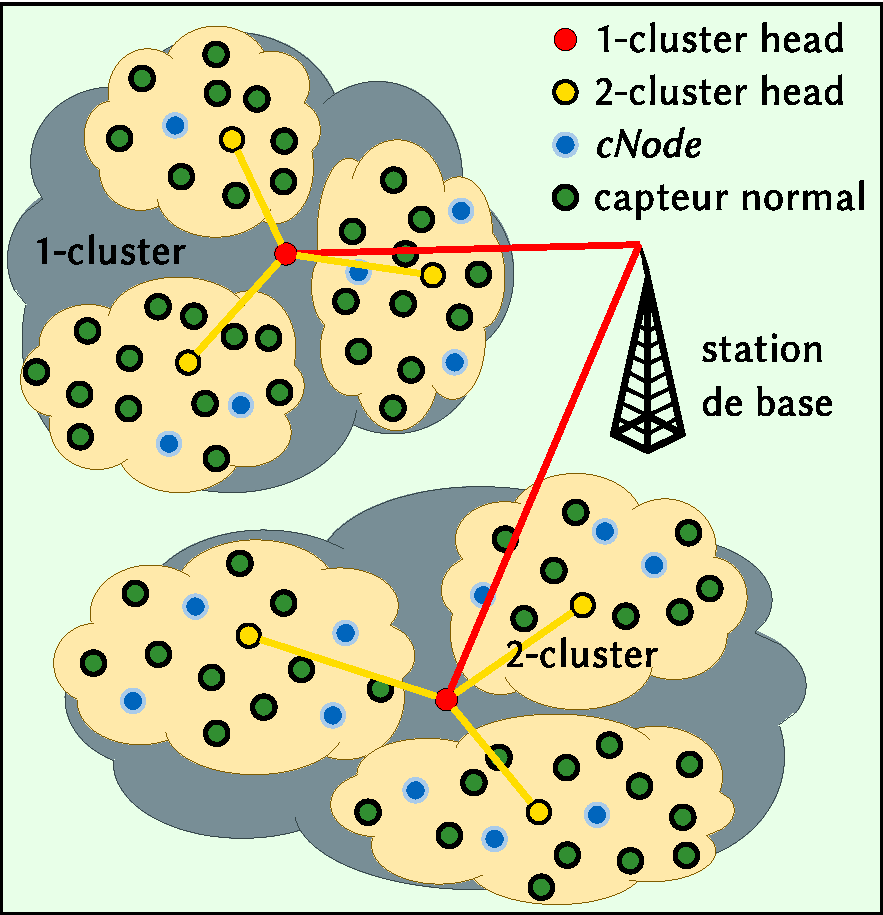
\includegraphics[width=.7\linewidth]{\chapterfig/2-clustered_network.pdf}
    \caption{Schéma du réseau avec deux niveaux de partition}\label{sa:fig:network}
\end{figure}
Ceci permet, à notre sens:
\begin{itemize}
    \item d'économiser davantage d'énergie par rapport à l'usage de \leach dans sa version simple;
    \item d'obtenir, en choisissant des nœuds de surveillance dans chacun des $2$-clusters, une meilleure couverture du réseau par les sentinelles, et de maximiser ainsi la probabilité de détection des nœuds compromis dans le réseau.
\end{itemize}
En pratique, $k$ doit être adapté en fonction du nombre de capteurs dans le réseau, de sa superficie, de la puissance et de la consommation énergétique des nœuds, et même des applications utilisées dans le réseau.
Des expériences ayant recours au matériel considéré sont indispensables pour déterminer les valeurs numériques optimales pour un réseau donné, ce qui empêche de fournir ici une estimation numérique: nous nous en tenons donc au degré $2$.

%===============================================================================
    \subsection{Des \cns pour surveiller le trafic}

La partition hiérarchique d'un réseau en clusters établit déjà une distinction entre deux rôles que peuvent assumer les capteurs: celui de nœud «normal», qui poursuit ses opérations de captage et de retransmission des données de façon classique, et celui de \ch, qui se retrouve chargé d'assurer la liaison entre les membres de son cluster et le restant du réseau.
À côté des nœuds «normaux» et des \chs, un troisième rôle va être attribué à certains capteurs, afin d'assurer la détection des attaques de type «\dds».
Certains capteurs se voient ainsi confier le rôle de «nœuds de contrôle», ici nommés \cns (introduits sous le nom de \textit{gNodes}\index{gNodes@\textit{gNodes}} dans~\cite{LC08}), et sont chargés de surveiller le trafic entrant et sortant des \chs.

Si un \cn constate qu'un capteur envoie, au cours d'une unité de temps, plus de données à leur \CH qu'une valeur de seuil déterminée $S_{\textrm{débit}}$, il retient que le nœud a eu un comportement anormal (il y a eu un écart important à la moyenne de la quantité de données envoyées par unité de temps).
Lorsque ce nœud réalise un certains nombres d'écarts, \cad lorsque le nombre de comportement anormaux détectés par un \cn dépasse une valeur de seuil $S_{\textrm{écarts}}$, le ou les nœuds de contrôle qui ont repéré ces écarts considèrent alors le capteur comme compromis.
Chaque \cn ayant détecté un nœud compromis envoie un message d'avertissement à son \ch.
Ici encore, un seuil $S_{\textrm{alertes}}$ est fixé pour le nombre minimum d'alertes qu'un \CH doit recevoir avant de considérer un nœud comme malveillant, et ce afin d'éviter qu'un nœud compromis se faisant passer pour un \cn ne déclare tous ses voisins comme compromis.
Plusieurs \cns distincts doivent donc détecter les écarts d'un nœud pour que celui-ci soit effectivement considéré comme compromis par le \ch.

Une fois que la malveillance d'un capteur est effectivement actée par un \ch, la charge incombe à ce dernier de prendre des mesures pour mitiger l'attaque.
En pratique, la solution utilisée ici est simple: tous les messages en provenance des nœuds considérés malveillants par le \ch sont ignorés (le \CH se met immédiatement à les ignorer, et il prévient les capteurs du cluster afin qu'ils puissent en faire autant).

Les \cns comparent également la taille des trafics entrant et sortant du \ch.
En cas d'écarts importants (en tenant compte des éventuels facteurs de compression des données et des messages ignorés des nœuds considérés compromis), ils peuvent être amenés à penser que le \ch est lui-même malveillant.
Dans ce cas, l'élection d'un nouveau \CH dans le cluster est déclenchée.

%===============================================================================
    \subsection{Sélection dynamique des \cns}

        \subsubsection{Motivations}
La partition du réseau permet de limiter aux seuls \chs les efforts énergétiques dus aux transmissions longues.
L'inconvénient est que, justement, ces \CH vont épuiser leur batterie beaucoup plus rapidement que s'ils étaient restés des nœuds ordinaires, tirant ainsi le réseau vers une fin de vie précoce.
Les nœuds ne sont pas toujours désignés \CH «à vie»: ainsi \leach renouvelle périodiquement la partition du réseau, choisissant à chaque itération de nouveaux \chs et entrainant la sélection d'un nouveau lot de \cns.

Mais tous les protocoles de \idx{clusterisation} ne prévoient pas nécessairement de renouvellement régulier de la partition.
De plus, s'ils n'émettent pas sur de longues distances, les \cns se retrouvent eux aussi à consommer plus d'énergie que les nœuds normaux, puisqu'il doivent sans cesse rester en écoute des transmissions qui les entourent, et analyser le débit de chacun de leurs voisins.
Pour répartir cette nouvelle charge, qui touche davantage de nœuds, nous proposons d'élire également les \cns de façon dynamique, sur une période plus courte que celle, éventuelle, qui correspond à la clusterisation du réseau.

Il est vrai que le renouvellement périodique des \cns rajoute des contraintes et augmente le volume des messages de contrôles à échanger dans le réseau.
Pour certaines applications des capteurs, ceci peut représenter un inconvénient que la répartition de la charge ne vient pas contrebalancer; mais de manière générale la préservation des réserves énergétiques est primordiale dans les \rcs, et un meilleur équilibre de la charge obtenu pour un prix relativement modeste ne semble pas superflu.
Autre remarque: en matière de détection d'intrusion, les \IDS les plus récents se vantent souvent de n'engendrer qu'un faible surplus de consommation dans le réseau~\cite{LZYP08}, et la question se pose donc de savoir si la répartition de la charge par un renouvellement dynamique reste pertinente; nous verrons en section suivante qu'avec un système aussi simple que nos \cns, les simulations annoncent un gain important sur la répartition de la charge.
Il faut également garder à l'esprit que les mécanismes de renouvellement périodique et de sélection des nœuds de surveillance ne sont pas dépendants du mécanisme de détection utilisé (\cad des \cns qui appliquent des règles sur le trafic analysé).
Ainsi, si un \IDS «concurrent»
\begin{itemize}
    \item présente une bonne capacité à économiser l'énergie du réseau,
    \item s'exécute seulement sur un sous-ensemble des nœuds du réseau,
    \item et ne nécessite pas, pour fonctionner, d'équipement distinct du matériel de base des capteurs,
\end{itemize}
alors la dynamique et les méthodes de sélection présentés dans cette thèse peuvent très bien être mis en œuvre pour optimiser détection et consommation.

Un dernier point reste à signaler.
Cette solution de renouvellement périodique améliore aussi la sécurité du réseau: si un attaquant cherche à compromettre tous les \cns du cluster, pour pouvoir poursuivre son attaque discrètement, le renouvellement dynamique apporte une parade efficace à l'attaque en complexifiant largement le nombre de cibles à corrompre.

        \subsubsection{Le choix par le hasard}
Le renouvellement périodique des capteurs de surveillance peut être réalisé de plusieurs façons.
Dans ce chapitre, une façon de faire très simple est employée: la sélection des \cns, pour chaque période, est ---~théoriquement~--- \idx{aléatoire}.
L'aléatoire est une notion délicate en informatique; nous nous contenterons plutôt d'un algorithme capable de générer des nombres dits «pseudo-aléatoires».
Une façon de procéder, par exemple, est de recourir à un algorithme capable de générer une suite de nombre d'apparence aléatoire, utilisés pour déterminer quels seront les \cns pour la période à venir~\cite{BMM13}.
Cet algorithme se doit de respecter les points suivants:
\begin{itemize}
    \item il doit nécessiter peu de calculs;
    \item sa période doit être grande;
    \item les valeurs générées doivent être indépendantes et distribuées uniformément.
\end{itemize}
Nous nous sommes tournés vers un type connu de générateurs, les \textit{Multiplicative Linear-Congruential Generators} (ou MLCG), qui possèdent effectivement une grande période~\cite{RJ91}.
\nomenclature{MLCG}{\textit{Multiplicative Linear-Congruential Generators}}
Plus précisément, le générateur retenu est de type $x_n = a\cdot x_{n-1}\bmod\ m$, où:
\begin{itemize}
    \item le nombre pseudo-aléatoire $x_n$ est généré à partir de son prédécesseur $x_{n-1}$;
    \item $m$ est de la forme $2^k$, ce qui facilite le calcul de $\bmod\ m$ (troncature à droite du résultat sur $k$ bits);
    \item $a$ doit être de la forme $8\cdot i\pm3$ (avec $i$ un entier positif) pour que le générateur ait la période maximale, égale à $2^{k-2}$;
    \item $x_0$ (la «graine», ou \textit{seed} en anglais) doit être un entier impair (toujours pour avoir la meilleure période).
\end{itemize}
La méthode de \textsc{Schrage}\index{methode de schrage@méthode de \textsc{Schrage}} permet de reformuler le générateur sous une forme qui prévient tout problème de débordement\,\footnote{Un débordement désigne le dépassement, au cours des calculs, de la valeur d'entier maximale gérée par le système, et se traduit par des erreurs de calcul.} lors de l'implémentation~\cite{RJ91}.
Le générateur est alors écrit sous la forme suivante: $a\cdot x\bmod m=g(x)+m\cdot h(x)$, avec:
\[\left\{
    \begin{aligned}
        g(x) & =a\cdot(x\bmod q)-r\cdot(x\mbox{~div~}q)\\
        h(x) & =(x\mbox{~div~}q)-(a\cdot x)\mbox{~div~}m\\
        q    & =m\mbox{~div~}a\\
        r    & =m\bmod a
    \end{aligned}
\right.\]
Voici finalement un exemple de générateur (il s'agit de celui qui a été implémenté pour réaliser les tests présentés en \sref{sa:sec:resultats}):
\[x_n=11\cdot x_{n-1}\bmod2^{16}\]
Sa période est égale à $2^{14}$.
Ce générateur peut alors être utilisé pour calculer des nombres pseudo-aléatoires allant de $0$ à $65535$ qui, ramenés sur le nombre attendu de \cns dans le cluster ou bien comparés à un seuil de probabilité, permettent de déterminer quels vont être les nœuds élus pour la période en cours.
Il convient naturellement d'attribuer une graine différente à chaque nœud du réseau, afin d'éviter que tous les nœuds produisent la même suite de nombres pseudo-aléatoires.
Ceci peut être réalisé en initialisant l'algorithme avec une mesure physique ---~après tout, il s'agit de capteurs!~--- dont la valeur est ramenée à l'entier impair le plus proche.

Mais une question subsiste: quelle va-t-être l'entité chargée d'exécuter cet algorithme et de procéder à l'élection des \cns?
Trois méthodes différentes sont ici proposées: une auto-élection distribuée, une élection centralisée au niveau des \CH, ou alors une élection centralisée au niveau de la \sdb.
%===============================================================================
    \subsection{Processus de sélection des \cns}

        \subsubsection{Auto-élection distribuée}
Une première solution consiste à réutiliser l'algorithme d'auto-désignation mis en œuvre par \leach, comme présenté sur la \figref{sa:fig:elecself}.
Chaque nœud non \CH choisit un nombre pseudo-aléatoire compris entre 0 et 1.
Si ce nombre est en-dessous du pourcentage de \cns désirés dans le réseau (et fixé au moment de l'implémentation par l'utilisateur), ce nœud devient un \cn.
Autrement, il reste un capteur normal.
\begin{figure}[ht]
    \centering
    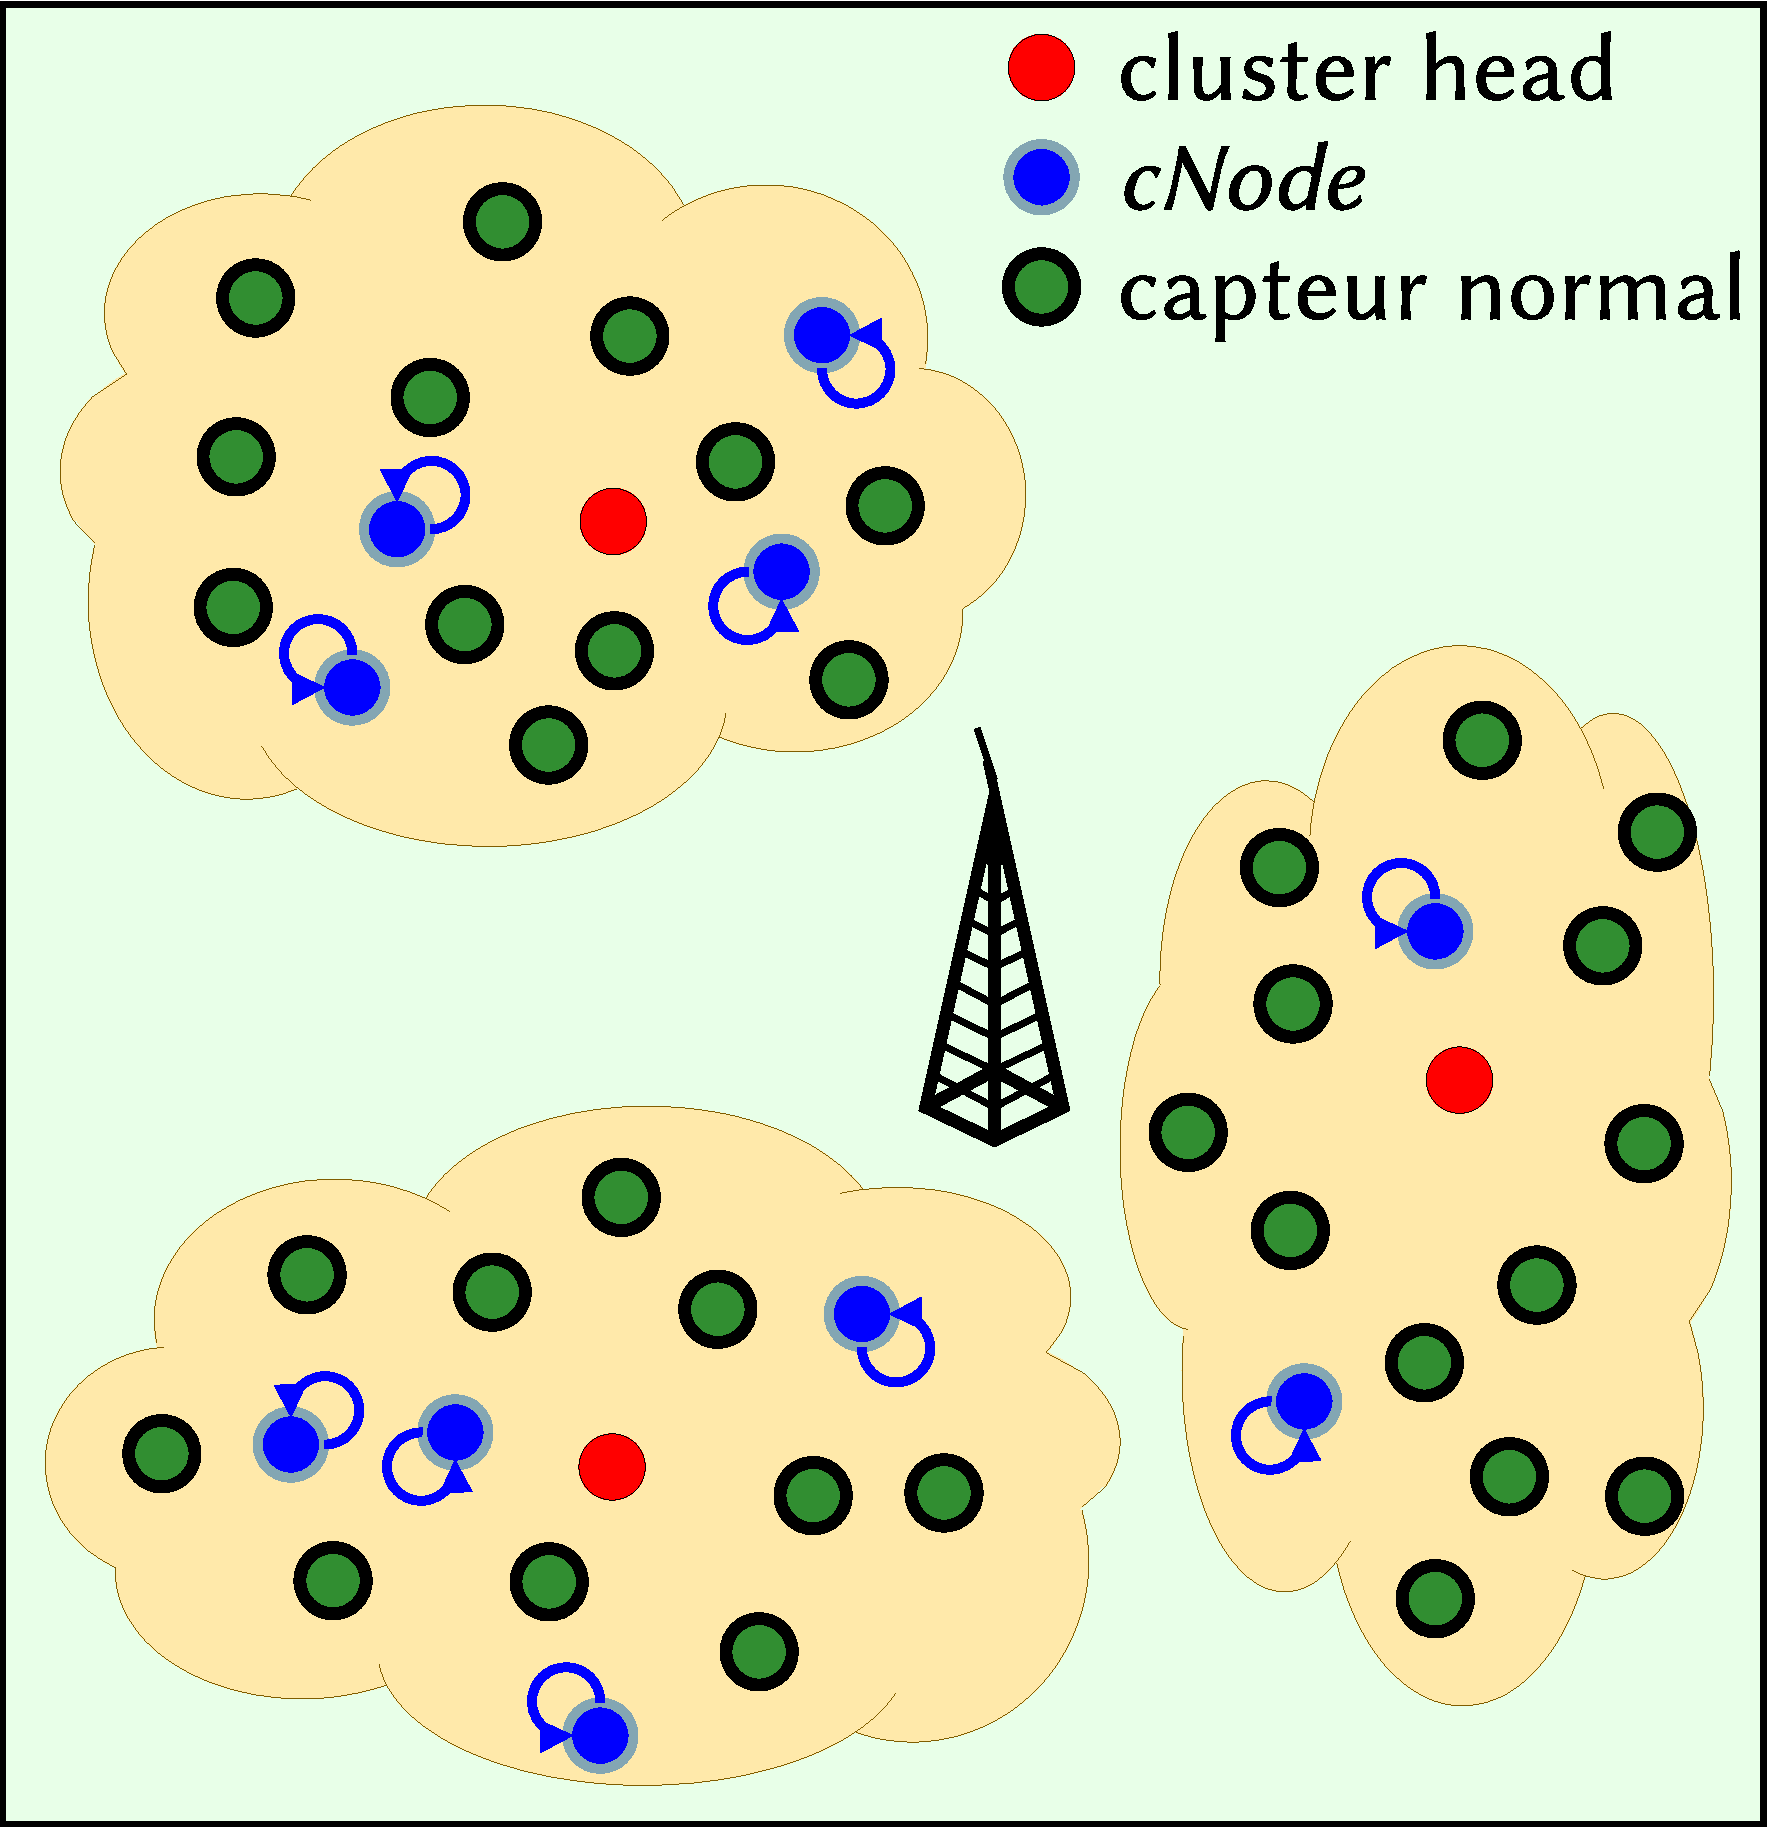
\includegraphics[width=.5\linewidth]{\chapterfig/elec_self.pdf}
    \caption{Auto-élection des \cns}\label{sa:fig:elecself}
\end{figure}

Cette méthode présente deux inconvénients.
Tout d'abord, elle impose à chaque nœud de calculer un nombre pseudo-aléatoire --- calcul parfois couteux ---, ce qui n'est pas nécessaire avec les deux autres méthodes.
Ensuite, chaque nœud choisit lui-même de se désigner (ou non) \cn, sans tenir compte de la décision de ses voisins.
Si bien que l'élection des \cns ne prend en compte à aucun moment la clusterisation du réseau.
Il est très peu probable que les \cns ainsi élus soient uniformément répartis entre les différents $2$-clusters du réseau.
Il est même possible que certains $2$-clusters se retrouvent totalement dépourvus de \cns (et se retrouvent ainsi dans l'incapacité de détecter une attaque).

Ce second point peut être contourné en menant une élection en deux étapes.
Dans un premier temps les nœuds choisissent d'endosser, ou non, le rôle de \cn; les \cns élus signalent alors leur statut au $2$-\CH auquel ils sont associés.
Au cours de la seconde étape, les $2$-\CH nomment des \cns supplémentaires dans leurs $2$-clusters respectifs si le nombre de signalements reçus au regard du nombre de nœuds dans les $2$-clusters est en-dessous d'un pourcentage minimal.

        \subsubsection{Élection centralisée au niveau des \chs}
La seconde méthode proposée consiste à décharger les nœuds classiques du processus d'auto-désignation, pour le remplacer par une nomination autoritaire réalisée par les $2$-\chs (voir \figref{sa:fig:elecch}).
Chaque \CH désigne alors un nombre de \cns correspondant au pourcentage indiqué par l'utilisateur.
Par exemple, si l'on souhaite obtenir dix pour cent de \cns, et qu'un $2$-cluster comporte cent capteurs, le \CH de ce cluster va produire dix nombres pseudo-aléatoires distincts qui seront associés aux identifiants de dix nœuds du cluster.
Le \CH envoie alors un message à chacun de ces dix nœuds pour leur ordonner de remplir le rôle de \cn sur la période en cours.
\begin{figure}[ht]
    \centering
    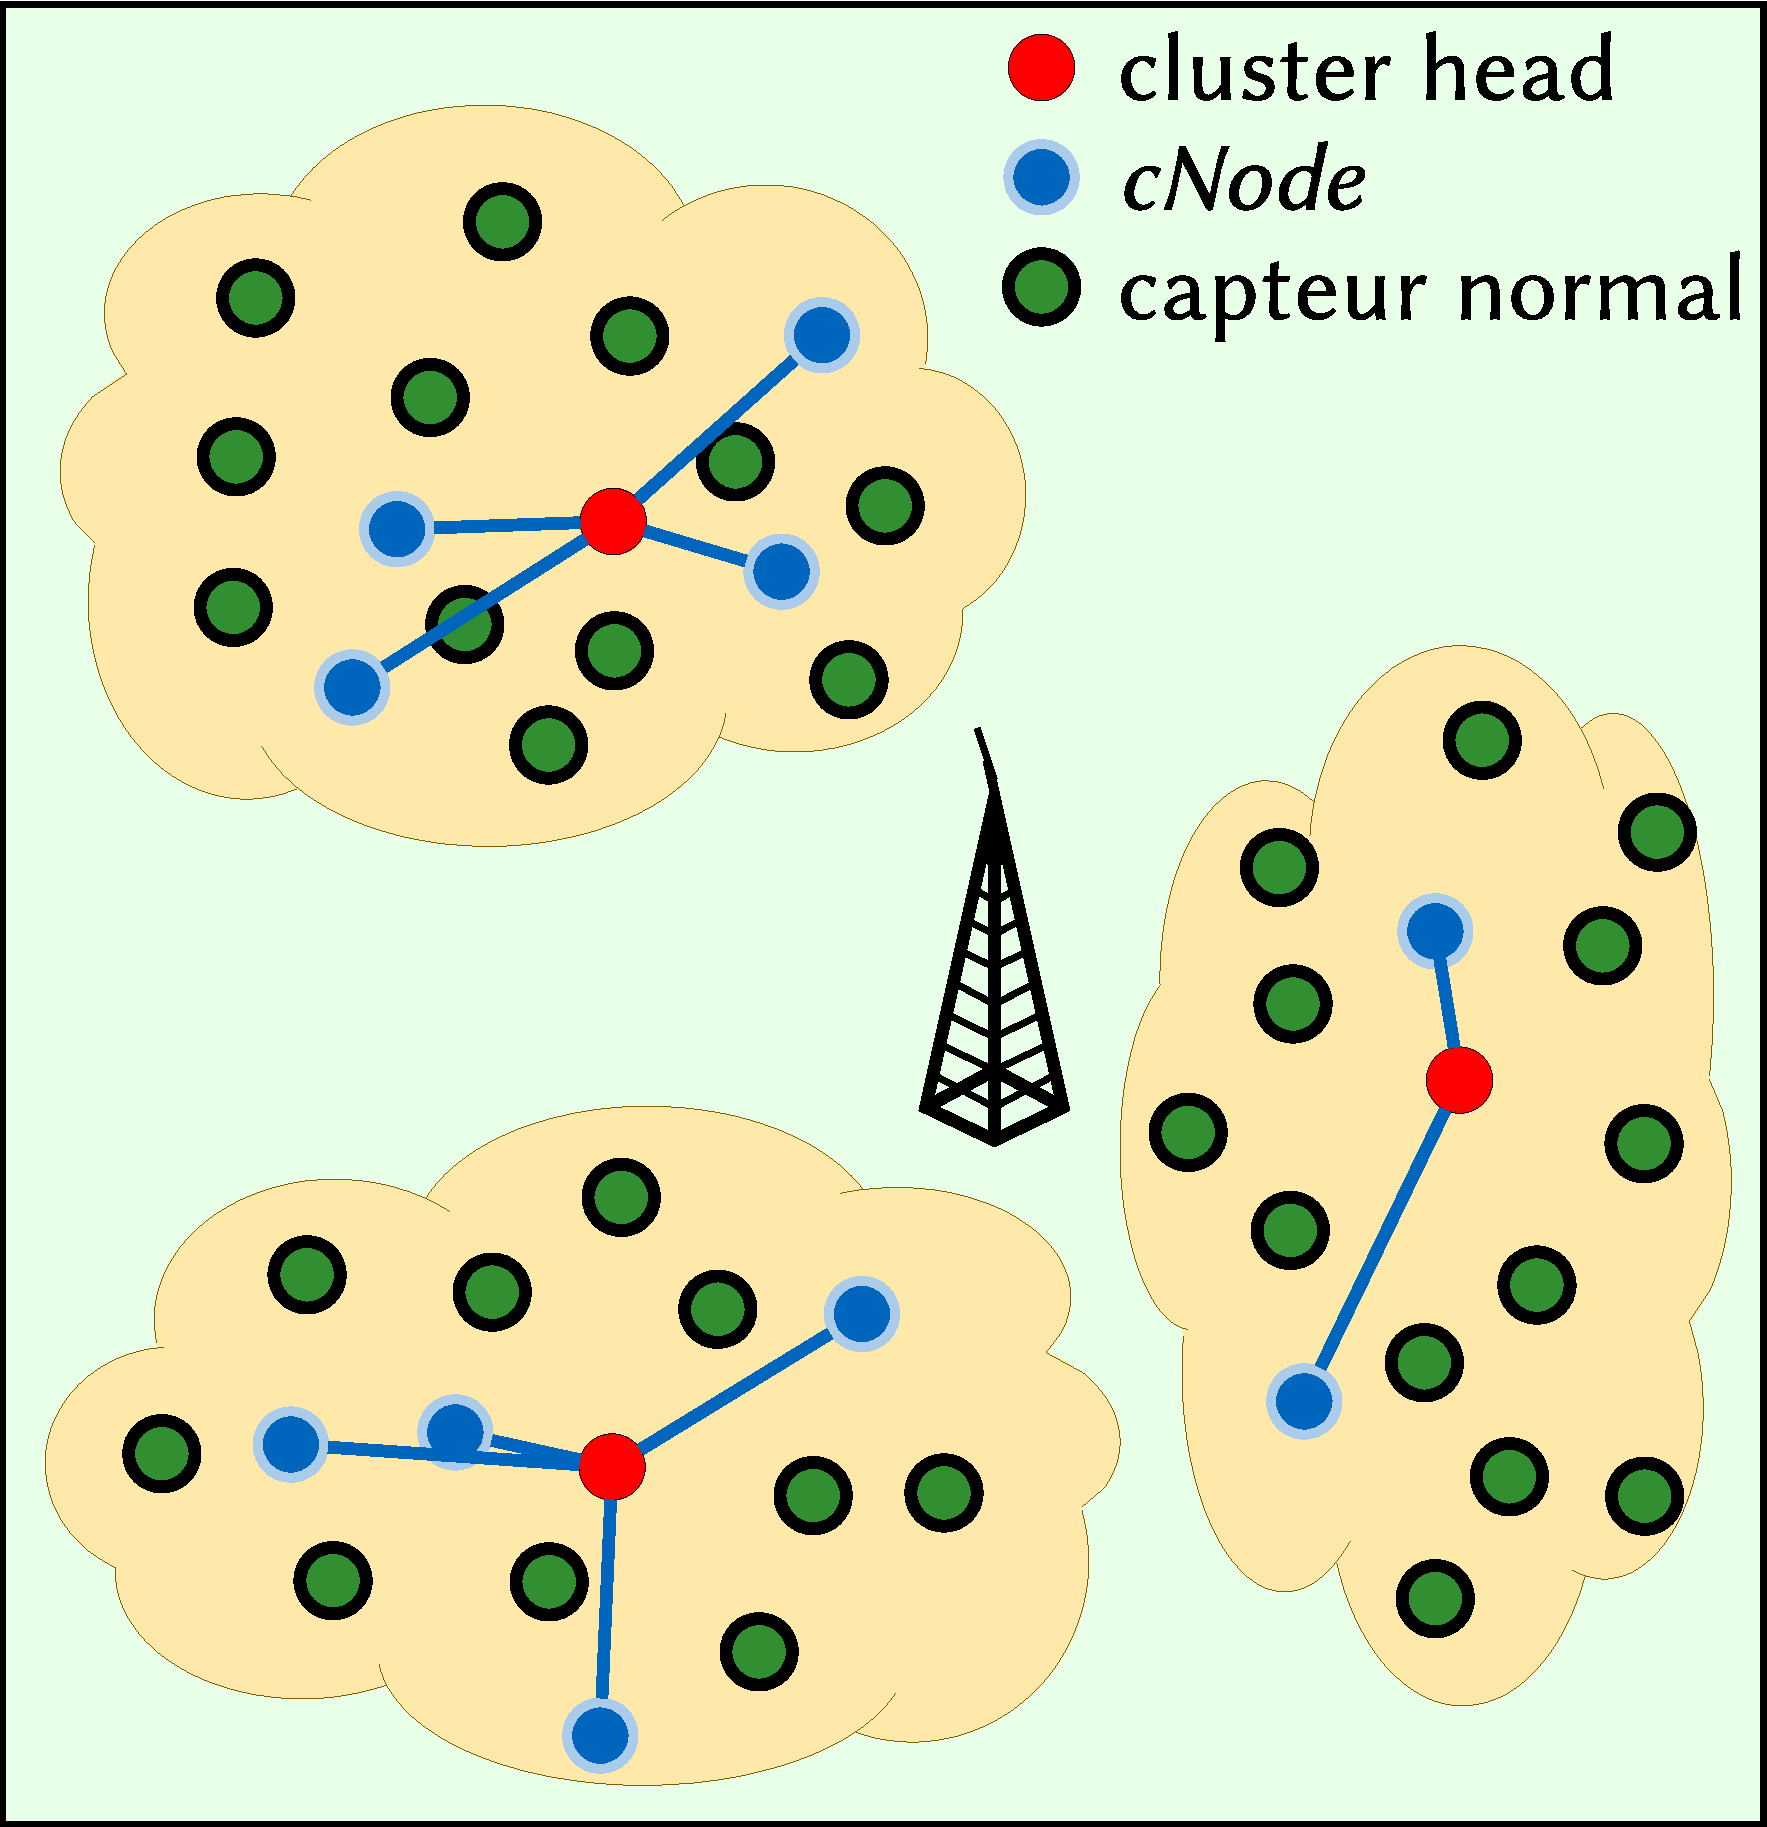
\includegraphics[width=.5\linewidth]{\chapterfig/elec_ch.pdf}
    \caption{Élection des \cns réalisée par les \chs}\label{sa:fig:elecch}
\end{figure}

Cette méthode est plus efficace en terme de calculs puisque seul les $2$-\CH ont à appliquer un algorithme de calcul de nombres pseudo-aléatoires.
Cependant, elle présente un autre désavantage: si l'un de ces \CH est compromis par un attaquant, il ne déclarera sans doute aucun \cn susceptible de le détecter, laissant ainsi tout son cluster à la merci d'autres attaques.
Comme l'algorithme \leach désigne à tour de rôle chaque capteur, sur un cycle complet, pour accomplir le rôle de \CH, tout nœud compromis deviendra logiquement \CH à un moment ou l'autre.
Le problème du \CH ne désignant aucun \cn peut donc légitimement se poser pour n'importe quel nœud compromis du réseau.
Qui plus est, il faut garder à l'esprit que rien n'empêche un nœud compromis de se déclarer \ch à chaque ronde de l'algorithme \leach.

Cette méthode est néanmoins celle qui est implémentée dans les travaux de la référence~\cite{GMT12}, et que nous reprenons pour nos tests (dont les résultats sont disponibles en \sref{sa:sec:resultats}).

        \subsubsection{Élection centralisée au niveau de la \sdb}
L'élection centralisée peut également être effectuée au niveau de la \sdb, comme représenté sur la \figref{sa:fig:elecbs}.
Les $2$-\CH du réseau font alors remonter à la \sdb la liste des nœuds de leurs $2$-clusters respectifs, et celle-ci retourne une liste de \cns pour chacun d'entre eux.
Les capacités (en mémoire, calcul, énergie) de la \sdb étant considérées comme illimitées, cette méthode a pour avantage de déporter toutes les tâches couteuses dans un environnement «sans contraintes».
Le calcul des nombres pseudo-aléatoires par la \sdb ne lui coute, pour ainsi dire, rien.
\begin{figure}[ht]
    \centering
    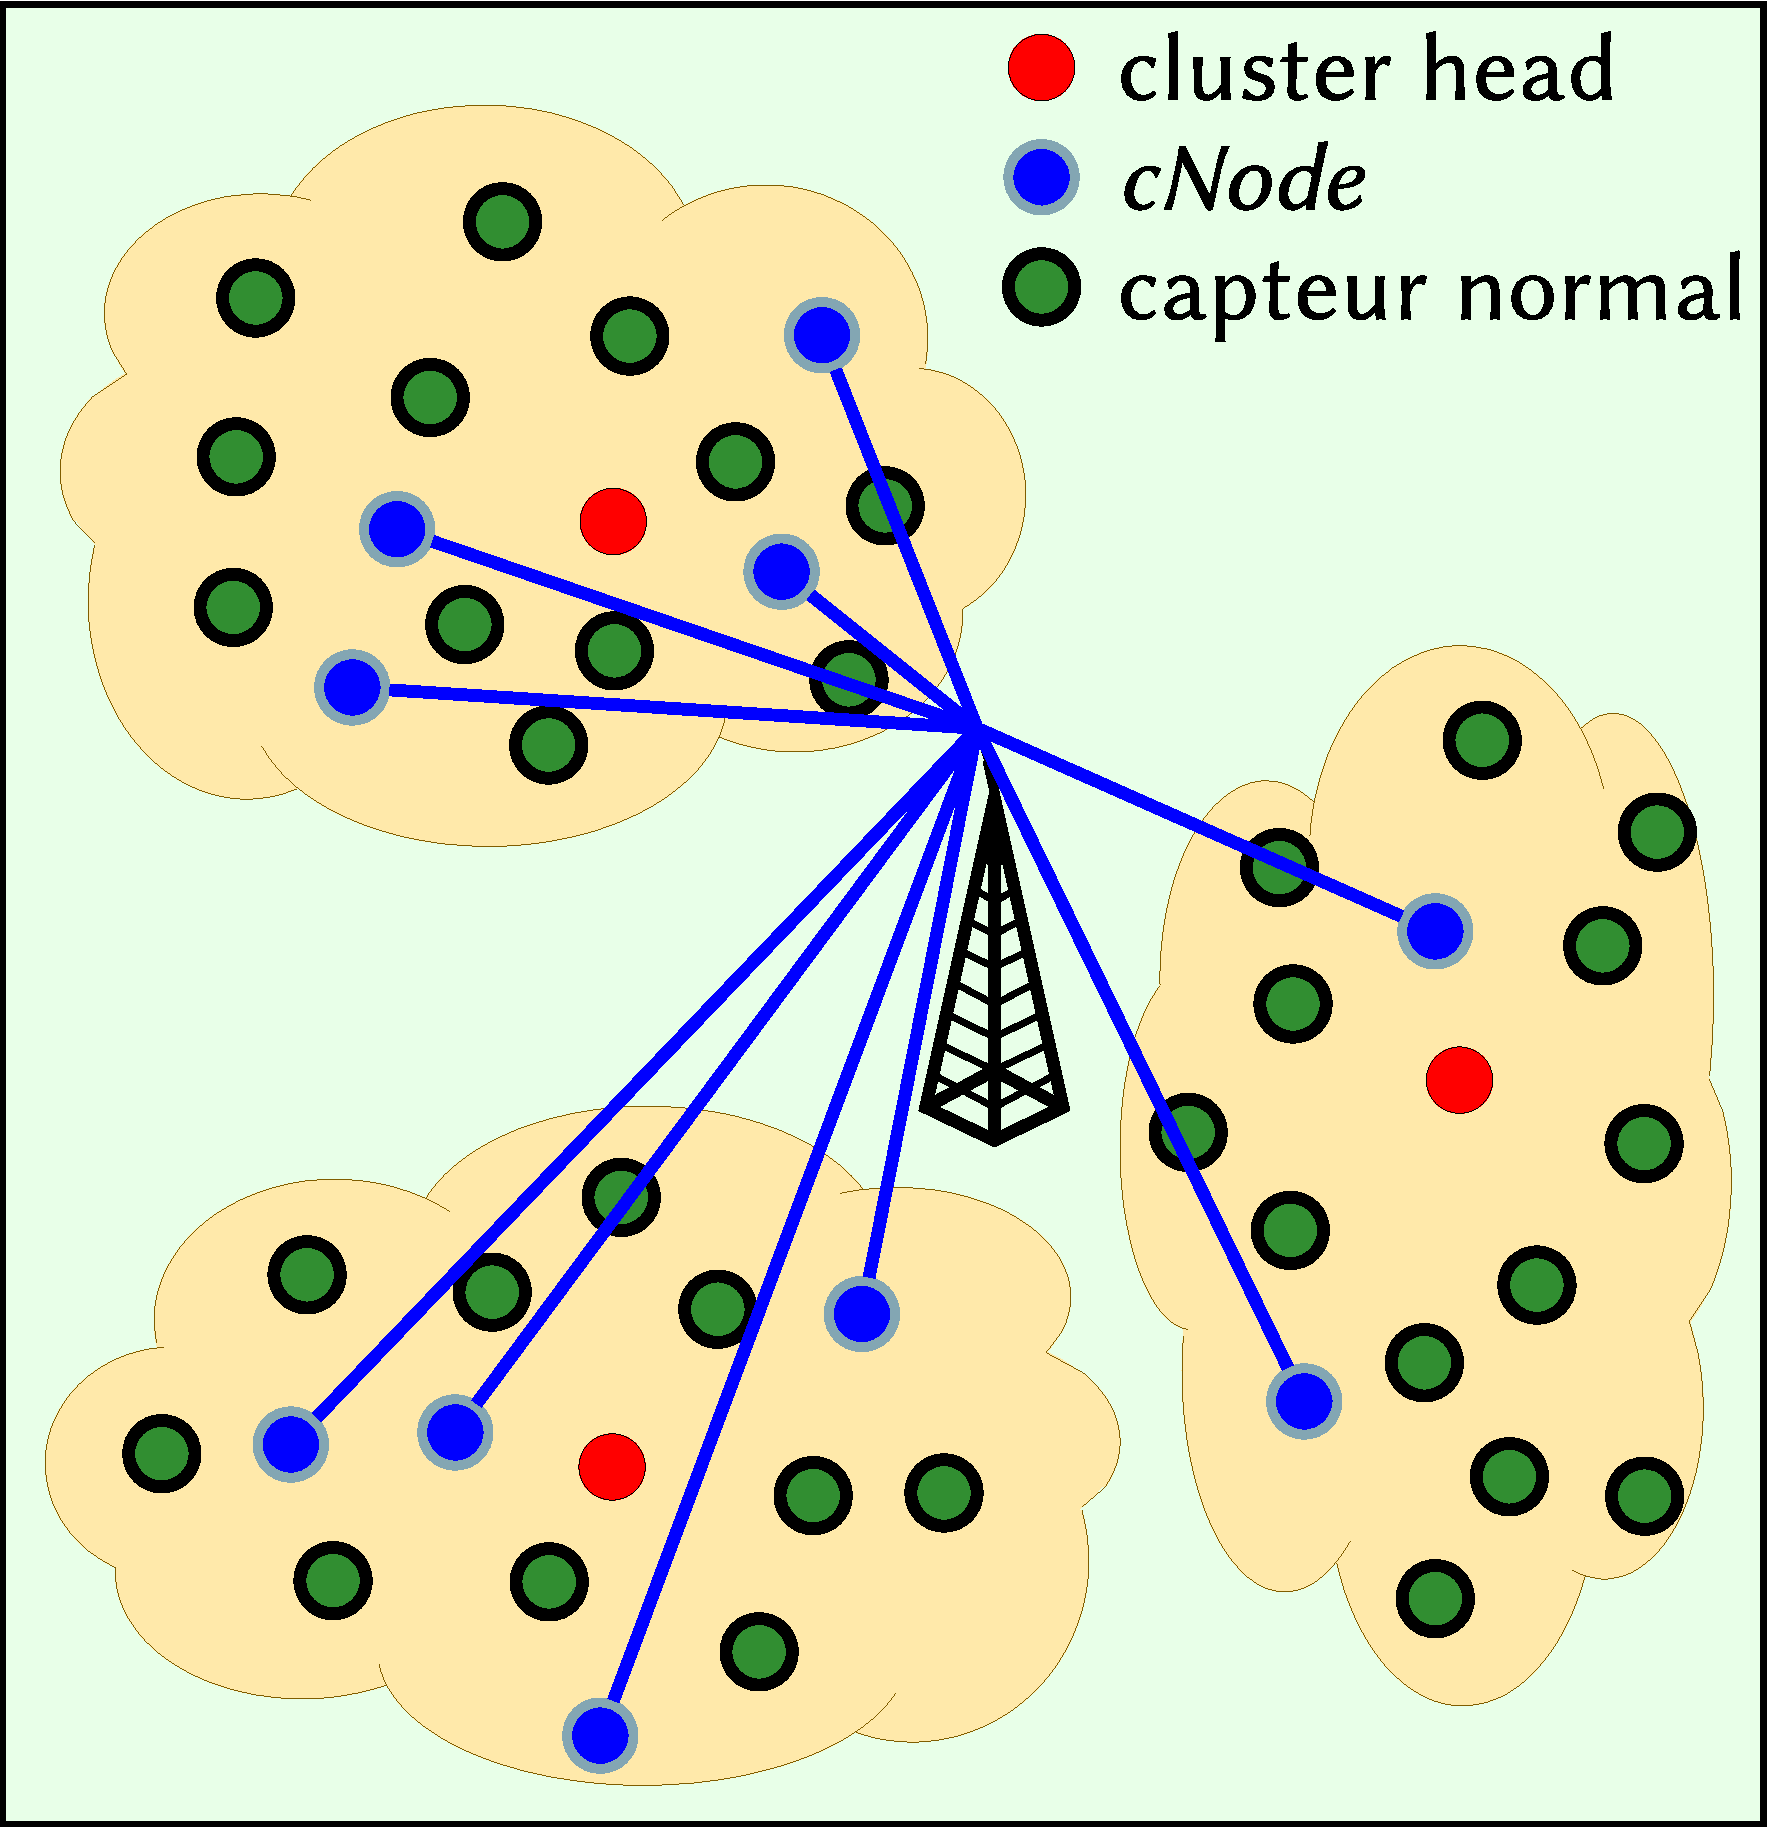
\includegraphics[width=.5\linewidth]{\chapterfig/elec_bs.pdf}
    \caption{Élection des \cns réalisée par la \sdb}\label{sa:fig:elecbs}
\end{figure}

En revanche cette méthode n'offre pas une meilleure fiabilité que la précédente.
Si un nœud compromis se déclare en temps que \CH, il risque fortement d'annoncer à la \sdb que son cluster est vide (il enverrait une liste vide en lieu et place de la liste des capteurs qui sont réellement présents dans son cluster).
Dans ce cas, la \sdb ne déclarera aucun \cn dans le cluster attaqué, et le \CH compromis ne sera pas détecté.
Pour parer à cette éventualité, la \sdb pourrait agir autrement lorsqu'elle reçoit une liste de capteurs vide.
Plus spécifiquement, elle devrait considérer que les nœuds dont elle n'a pas eu de nouvelles \via les listes des \CH ne sont peut-être pas simplement morts, mais escamotés par un \ch corrompu.
Ces nœuds disparus devraient donc être considérés comme potentiellement éligibles, de sorte que certains d'entre eux au moins soient déclarés \cns.

L'inconvénient majeur de cette méthode est le fait que la nature distribuée de l'élection (avec tous les avantages qu'apporte un algorithme distribué) est complètement
perdue.

Les avantages et inconvénients de chacune de ces trois méthodes présentées sont résumés dans la \tabref{sa:table:elec}.
\begin{table}[ht]
    \caption{Avantages et inconvénients de chaque méthode}\label{sa:table:elec}
    \medskip
    \begin{small}
        \begin{tabular}{m{.19\textwidth} m{.35\textwidth} m{.35\textwidth}}
            \toprule
            \centering \textsc{Méthode} & \centering \textsc{Avantages} & \centering \textsc{Inconvénients} \tabularnewline
            \midrule
            \centering Auto-élection des \cns (selon le modèle de \leach)    & %
                \textbullet~Très simple à mettre en œuvre\newline%
                \textbullet~Pas d'envoi de paquets à travers le réseau pour désigner les \cns%
                & %
                \textbullet~Chaque nœud doit calculer un nombre pseudo-aléatoire\newline%
                \textbullet~Ne tient pas compte de la topologie du réseau\tabularnewline
            \midrule
            \centering Élection des \cns par les \ch                        & %
                \textbullet~Seuls les \CH calculent les nombres pseudo-aléatoires%
                & %
                \textbullet~Si le \CH est compromis, il ne désigne aucun \cn (un nœud compromis peut se déclarer \CH à chaque ronde de \leach)\tabularnewline
            \midrule
            \centering Élection des \cns par la \sdb                & %
                \textbullet~Aucun calcul réalisé par les nœuds\newline%
                \textbullet~Distribution spatiale idéale des \cns%
                & %
                \textbullet~Si le \CH est compromis, il déclare un cluster vide\newline%
                \textbullet~Perte de l'aspect centralisé de l'algorithme\tabularnewline
            \bottomrule
        \end{tabular}
    \end{small}
\end{table}


% vim: set spelllang=fr foldmethod=marker:
\section{Modélisation}
\label{sa:sec:modelisation}

Nous avons détaillé la solution proposée. À présent, nous allons présenter plusieurs modèles possibles permettant de représenter cette solution, et d'en évaluer les performances selon divers critères.

%===============================================================================
    \subsection{Chaines de Markov}

        \subsubsection{Présentation et hypothèses de travail}
Nous avons modélisé notre solution sous la forme d'un processus de Markov à temps continu (CMTC, pour chaine de Markov à temps continu).

Notre modèle représente un cluster d'un réseau de capteurs sans fil qui vérifie les hypothèses suivantes:
\begin{itemize}
    \item seul le cluster est modélisé;
    \item le cluster contient exactement un \CH, $s$ capteurs chargés d'effectuer des mesures, et $m$ nœuds jouant le rôle de \cns\footnote{$s$ pour \textit{sensing node}, $m$ pour \textit{monitoring node}.};
    \item il existe exactement un nœud compromis parmi les $s$ capteurs;
    \item le capteur $i$ ($1 \leq i \leq s$) génère du trafic selon un processus de Poisson de paramètre $\lambda_i$;
    \item le nœud compromis $c$ génère du trafic selon un processus de Poisson de paramètre $\lambda_i$ (tel que $\forall i\in[\![1;s]\!]\backslash\{c\},\; \lambda_c\gg\lambda_i$);
    \item chaque \cn effectue une détection du trafic environnant de façon périodique, selon une distribution exponentielle de paramètre $\mu$; si un trafic anormal est observé, le \cn transmet un rapport d'anomalie au \CH;
    \item la topologie du cluster correspond à un graphe connexe: chaque nœud peut atteindre directement chacun des autres nœuds du cluster.
\end{itemize}

        \subsubsection{Modélisation}
Sous les hypothèses précédentes, notre modèle peut être représenté par une CMTC multi-dimensionnelle de taille $m$.
Il est alors exprimé sous la forme d'un $m$-uplet $x\!=\!(x_1,x_2,\dots,x_m)$ de macro-états $x_k\!=\!(x_{k_1},x_{k_2},\dots,x_{k_s},x_{k_d})$.
Chaque macro-état $x_k$    garde en mémoire le nombre de paquets détectés par le \cn $k$ ($1\leq k\leq m$).
Plus exactement, chaque $x_{k_i}$ ($1\leq i\leq s$) est un compteur, initialisé à $0$, qui est incrémenté à chaque fois que le \cn $k$ détecte un paquet en provenance du capteur $i$.
$x_{k_d}$ est une variable de type booléen, initialisée à $0$, et passée à $1$ lorsque le \cn $k$ détecte un trafic anormalement élevé.
La fonction de seuil $f:s^s\rightarrow\{0;1\}$ est utilisée par les \cns pour déterminer la nature normale ou non du trafic (elle indique si un paquet a dépassé ou non le seuil des communications dites «~normales~»).
Elle prend pour argument les valeurs des $s$ compteurs $x_{k_1},x_{k_2},\dots,x_{k_s}$ d'un macro-état $x_k$ associé à un \cn $k$, et la valeur retournée est stockée dans $x_{k_d}$.

Voici un exemple d'équation de transition pour un macro-état générique $x_k$, $1\leq k\leq m$.
Le macro-état $x$, représentant l'intégralité du système, est directement obtenu en agrégeant les différents $x_k$.
Le compteur $x_{k_c}$ représente dans la suite le nombre de messages émis par le nœud compromis et captés par le \cn $k$.
L'équation est donnée en figure~\ref{sa:fig:eqtrans}

\newlength{\fboxlinelen}
\setlength{\fboxlinelen}{\linewidth}
\addtolength{\fboxlinelen}{-4\fboxsep}
\addtolength{\fboxlinelen}{-2\fboxrule}

\begin{figure}[H]
    \fbox{
        \begin{minipage}{\fboxlinelen}
            \begin{eqnarray*}
                x_k    & \rightarrow & \mbox{Transmission d'un capteur normal} \\
                    & \rightarrow & (x_{k_1},\dots,x_{k_i}+1,\dots,x_{k_c},  \dots,x_{k_s},0) \\
                    &             & \qquad\mbox{avec la fréquence }\lambda_{i}\!\neq\!\lambda_{c} \\ \\
                    & \rightarrow & \mbox{Transmission du nœud compromis} \\
                    & \rightarrow & (x_{k_1},\dots,x_{k_i},  \dots,x_{k_c}+1,\dots,x_{k_s},0) \\
                    &             & \qquad\mbox{avec la fréquence }\lambda_{c}\\ \\
                    & \rightarrow & \mbox{Vérification; détection d'un trafic anormal}\\
                    & \rightarrow & (0,\dots,0,\dots,0,\dots,0,1) \\
                    &             & \qquad\mbox{avec la fréquence }\mu \cdot 1_{f(x_k)\geq \mathit{seuil}} \\ \\
                    & \rightarrow & \mbox{Vérification; aucun trafic anormal détecté} \\
                    & \rightarrow & (0,\dots,0,\dots,0,\dots,0,0)  \\
                    &             & \qquad\mbox{avec la fréquence }\mu \cdot 1_{f(x_k)<\mathit{seuil}}
            \end{eqnarray*}
        \end{minipage}
    }
    \caption{Équation de transition du processus de Markov à temps continu modélisant le cluster}\label{sa:fig:eqtrans}
\end{figure}

\bigskip
Formulé autrement: le \cn $k$, dans l'état $x_k$, reçoit périodiquement les messages de chaque capteur $i$ ($1\leq i\leq s, i\!\neq\!s$): ce sont des transmissions dites «~normales~», qui surviennent avec une fréquence moyenne $\lambda_i$.
Chaque message reçu laisse le \cn $k$ dans un état presque identique, à la seule différence que le compteur $x_{k_i}$ est incrémenté de $1$.
La même chose se produit avec une fréquence $\lambda_c$ pour les messages envoyés par le nœud compromis, qui provoque à chaque fois l'incrémentation du compteur $x_{k_c}$.
Enfin, la vérification du trafic enregistré par le \cn $k$ survient avec une fréquence $\mu$.
La fonction $f$ est appliquée sur l'ensemble des $x_{k_i}$, $i$ allant de $1$ à $s$.
Si l'un des capteurs a envoyé un nombre de paquets supérieur à la valeur de seuil (\cad si l'on a $f(x_k)\geq \mathit{seuil}$), le drapeau $x_{k_d}$ est levé.
Un message d'alerte est alors envoyé du \cn $k$ au \ch.
Si, en revanche, aucune anomalie n'est à rapporter, le drapeau $x_{k_i}$ est laissé à $0$, et rien n'est envoyé.
Dans les deux cas, tous les compteurs $x_{k_i}$ sont réinitialisés à $0$, afin que la prochaine vérification soit effectuée sur des données «~fraiches~» (et pour ne pas déclencher par erreur une fausse détection par cumul des nombres de paquets envoyés d'une période sur l'autre).

La probabilité de détection du nœud compromis par le \cn $k$, notée $\Delta_k$, est la suivante:
\[\Delta_k=\sum_{x_{k_1},\dots,x_{k_s}}^\infty\pi(x_{k_1},\dots,x_{k_s},x_{k_d}=1)\]
où $\pi(x_{k_1},x_{k_2},\dots,x_{k_{s}},x_{k_d})$ représente la distribution stationnaire du macro-état $x_k\!=\!(x_{k_1},x_{k_2},\dots,x_{k_{s}},x_{k_d})$.

        \subsubsection{Limites du modèle}
Représenté sous la forme d'un processus de Markov à temps continu, le modèle suppose que la période séparant deux vérifications consécutives du trafic par un \cn est une variable aléatoire qui suit une distribution exponentielle.
Il s'agit là d'une approximation grossière; en réalité, la vérification intervient à intervalles réguliers (de longueur fixe), voire même en continu.
Il est donc nécessaire de choisir d'autres systèmes que les processus de Markov pour modéliser notre solution avec plus de précision.
Nous allons nous tourner par exemple vers des processus non-markoviens, qui ne présentent pas cette contrainte.

%===============================================================================
    \subsection{Réseaux de Petri}
Une autre représentation possible de notre système passe ainsi par l'utilisation de processus stochastiques à évènements discrets (PSED, ou DESP, \textit{Discrete-Event Stochastic Processes}, ou encore \textit{Generalized Semi-Markov Processes}).
Leur avantage principal sur les processus de Markov est leur capacité à représenter des événements dont la distribution n'est pas nécessairement exponentielle.
Plus particulièrement, nous allons utiliser des réseaux de Petri stochastiques généralisés étendus.

        \subsubsection{Présentation des réseaux de Petri stochastiques généralisés étendus}
\label{sa:subsubsec:presRPSGE}
Les réseaux de Petri stochastiques généralisés (RPSG) sont une classe de réseaux de Petri destinée à modéliser des processus stochastiques.
Leur version étendue (RPSGE) permet de représenter des transitions dont les délais sont distribués de façon quelconque~\cite{ABCDF95}.
Il s'agit d'un langage de haut niveau permettant de représenter des processus stochastiques à événements discrets (PSED, ou processus semi-markoviens généralisés, PSMG), qui au contraire des processus markoviens «~classiques~» ne sont pas limités à la représentation d'événements à distribution exponentielle.
RPSGE reprend, à quelques différences près, les définitions, la syntaxe et la représentation graphique des réseaux de Petri classiques, enrichis par des propriétés supplémentaires portant sur les transitions.
Ces dernières sont dites soit \textit{immédiates}, soit \textit{minutées}.
Elles sont de plus caractérisées par les éléments suivants:
\begin{enumerate}
    \item une distribution qui détermine de façon aléatoire le délai écoulé avant que la transition ne soit franchie;
    \item une priorité qui établit de façon déterministe la transition à franchir en premier, en cas d'égalité;
    \item un poids qui est utilisé pour tirer de façon aléatoire la transition à franchir en premier, en cas de conflits sur le délai écoulé et sur les priorités.
\end{enumerate}

Nous utilisons deux types de transitions minutées:
\begin{itemize}
    \item les distributions minutées exponentiellement distribuées (marquées dans les figures qui suivent par des rectangles vides, voir par exemple la transition \textsf{T1} sur l'exemple de gauche de la figure~\ref{sa:fig:gspnex1});
    \item les distributions minutées distribuées de façon déterministe (marquées dans les figures qui suivent par des rectangles bleus, voir par exemple la transition \textsf{T1} sur l'exemple de droite de la figure~\ref{sa:fig:gspnex1}).
\end{itemize}
Les transitions immédiates sont marquées par des rectangles pleins et noirs (voir par exemple la transition \textsf{T2} dans les exemples de la figure~\ref{sa:fig:gspnex1}).
Nous avons aussi recours à des arcs inhibiteurs.
Il s'agit d'arêtes dont la flèche sur les représentations graphiques est remplacée par un cercle (par exemple, l'arc reliant la place \textsf{P1} à la transition \textsf{T2} dans l'exemple de droite de la figure~\ref{sa:fig:gspnex1}), et accompagnées d'un chiffre.
Les règles de franchissement des transitions sont légèrement différentes avec ces arcs, puisque ces franchissement ne peuvent être effectués que si le nombre de jetons en amont de la transition est strictement inférieur au nombre indiqué sur l'arc.
Par exemple, sur la partie droite de la figure~\ref{sa:fig:gspnex1}, la transition \textsf{T2} peut être franchie, car \textsf{P1} ne contient que deux jetons (on a bien $2<3$).
\begin{figure}[H]
    \centering
    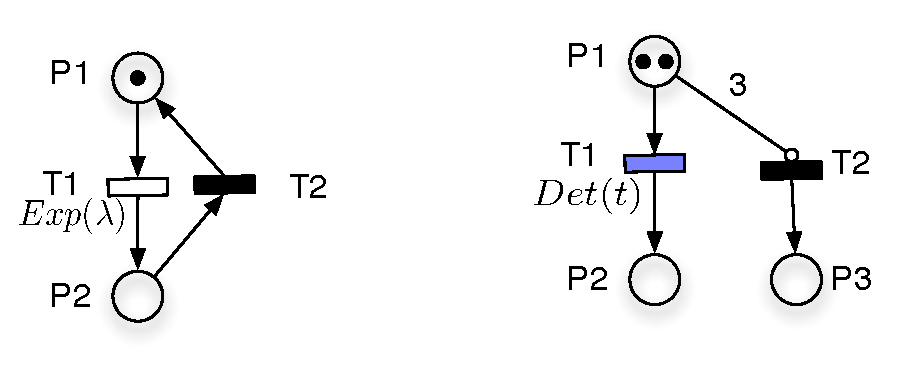
\includegraphics[width=.8\linewidth]{\chapterfig/GSPNex1.pdf}
    \caption{Exemples simples d'eGSPN: transitions immédiates, transition minutée et arcs inhibiteurs}\label{sa:fig:gspnex1}
\end{figure}

        \subsubsection{Modélisation des nœuds}
Nous allons procéder par étapes en modélisant:
\begin{enumerate}
    \item les nœuds capteurs «~simples~»;
    \item les \cns élus de manière statique;
    \item les \cns élus de manière dynamique (dont la modélisation diffère légèrement).
\end{enumerate}

            \paragraph{Modélisation des capteurs simples}
Le comportement des capteurs basiques est simple: chaque capteur $i$ envoie des paquets selon un processus de Poisson de paramètre $\lambda_i$.
Ce comportement est modélisé par le RPSG présenté en figure~\ref{sa:fig:snodegspn}.
\begin{figure}[H]
    \centering
    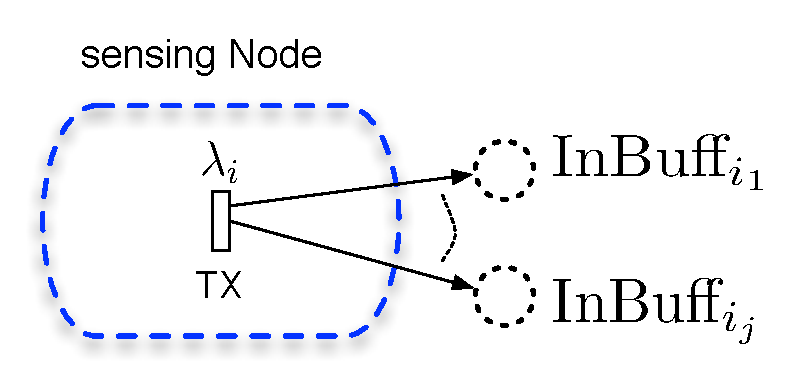
\includegraphics[width=.5\linewidth]{\chapterfig/sNode_GSPN.pdf}
    \caption{Modèle RPSG d'un nœud capteur simple}\label{sa:fig:snodegspn}
\end{figure}
Le nœud est symbolisé par les pointillés bleus.
Dans ce nœud $i$ se trouve une unique transition \textsf{TX}, sans place en entrée, autrement dit: toujours active.
Elle est minutée, avec une distribution exponentielle de paramètre $\lambda_i$: chaque événement correspond à l'envoi de jetons sur tous ses arcs sortants.
Ces arcs sont rattachés à la place \textsf{InBuff$_{i_j}$} de chacun des nœuds voisins du nœud $i$ (on trouve donc autant d'arcs sortants que de nœuds voisins).
L'intégralité de la fonction de mesure et d'envoi des données utiles du réseau de capteurs peut être modélisée par plusieurs éléments représentés par ce «~modèle de nœud~».
Un nœud compromis $c$ sera également représenté selon le même modèle, avec un paramètre $\lambda_c$ plus élevé que les autres $\lambda_i$.

            \paragraph{Modélisation des \cns élus de façon statique}
Un \cn élu de façon statique joue uniquement son rôle de \cn: il monitore le trafic, mais n'effectue pas de mesure sur son environnement.
Le modèle RPSGE associé à ce type de nœud est présenté en figure~\ref{sa:fig:cnodegspn1}.
\begin{figure}[H]
    \centering
    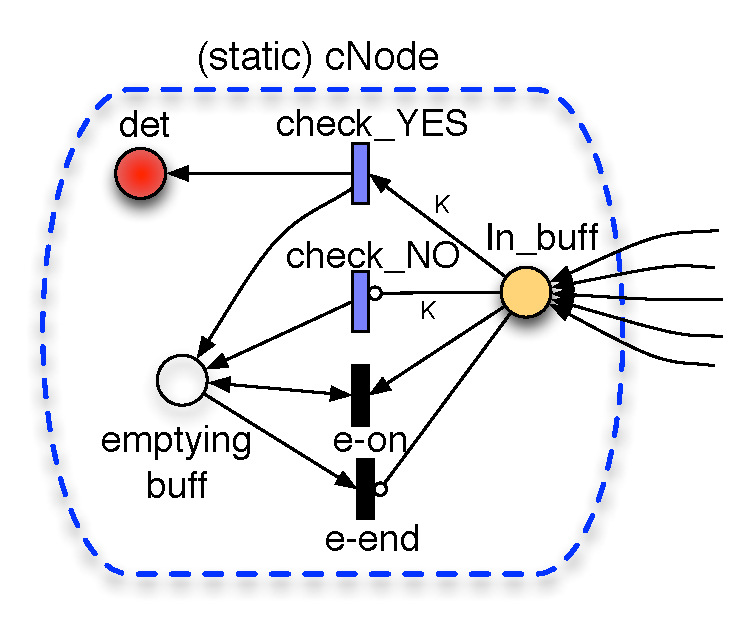
\includegraphics[width=.6\linewidth]{\chapterfig/cNode_GSPN.pdf}
    \caption{Modèle RPSGE d'un \cn élu de manière \emph{statique}}\label{sa:fig:cnodegspn1}
\end{figure}
La place \textsf{In\_buff} représente le tampon contenant les messages reçu par le nœud.
Un jeton arrivant dans cette place (depuis un nœud «~normal~») représente un message capté par le \cn\footnote{En réalité, il devrait y avoir une place \textsf{In\_buff$_i$} distincte pour les jetons provenant de chaque nœud voisin $i$ du \cn. Pour simplifier la représentation, tous les jetons arrivant au modèle du nœud sont rassemblés dans une place unique.}.
La vérification du respect de la valeur seuil $K$ pour le trafic est réalisée à intervalles de temps constants.
Les transitions \textsf{check\_YES} et \textsf{check\_NO} sont «~activées~» au bout de chaque période, et servent à assurer la vérification.
S'il y a au moins $K$ jetons dans la place, la transition \textsf{check\_YES} est franchie.
Un jeton est alors placé dans la place \textsf{det}, et fait en quelque sorte office de drapeau levé pour indiquer la détection d'un trafic anormal.
L'arrivée d'un jeton dans la place \textsf{det} déclenche l'envoi d'un message d'alerte au \ch.
Si, en revanche, il y a moins de $K$ jetons dans la place \textsf{In\_buff}, aucun jeton n'est produit dans la place \textsf{det}.
Dans un cas comme dans l'autre, la place \textsf{emptying~buff} reçoit un jeton (soit par \textsf{check\_YES}, soit pat \textsf{check\_NO}).
Un jeton dans cette place permet de vider le tampon \textsf{In\_buff}: la transition \textsf{e-on} consomme le jeton de la place \textsf{emptying~buff}, et un jeton de \textsf{In\_buff}.
Un nouveau jeton est créé dans \textsf{emptying~buff}.
Le processus est répété jusqu'à ce que la place \textsf{In\_buff} soit vide; dans ce cas, la transition \textsf{e-end} est franchie et ne produit rien, mais met fin à la consommation des jetons.
Les étapes permettant de vider le tampon ne consomment pas de temps, et permettent de repartir avec un compteur neutre pour la période qui mènera à la vérifiation suivante.

            \paragraph{Modélisation des \cns élus de façon statique}
Le modèle RPSGE représentant le \cn élu de façon dynamique ressemble à son homologue élu de façon statique.
Cependant, en raison de l'élection dynamique, tous les nœuds vont assumer périodiquement le rôle de \cn et le rôle de capteur simple.
Il est donc nécessaire d'ajouter, aux places et transitions des précédents \cns, une place \textsf{cNode} ainsi qu'une transition toujours autorisée, associée à une distribution exponentielle.
La première permet d'indiquer à chaque instant si le nœud joue le rôle de \cn (si la place contient un jeton) ou bien de capteur simple (cas contraire).
La seconde permet de produire des jetons selon un processus de Poisson lorsque le nœud fait office de capteur simple (dans ce cas la place \textsf{cNode} est vide et l'arc inhibiteur autorise le franchissement de la transition \textsf{TX}; le nœud se comporte exactement comme avec le modèle de la figure~\ref{sa:fig:snodegspn}).
Le modèle est représenté sur la figure~\ref{sa:fig:cnodegspn2}.
\begin{figure}[H]
    \centering
    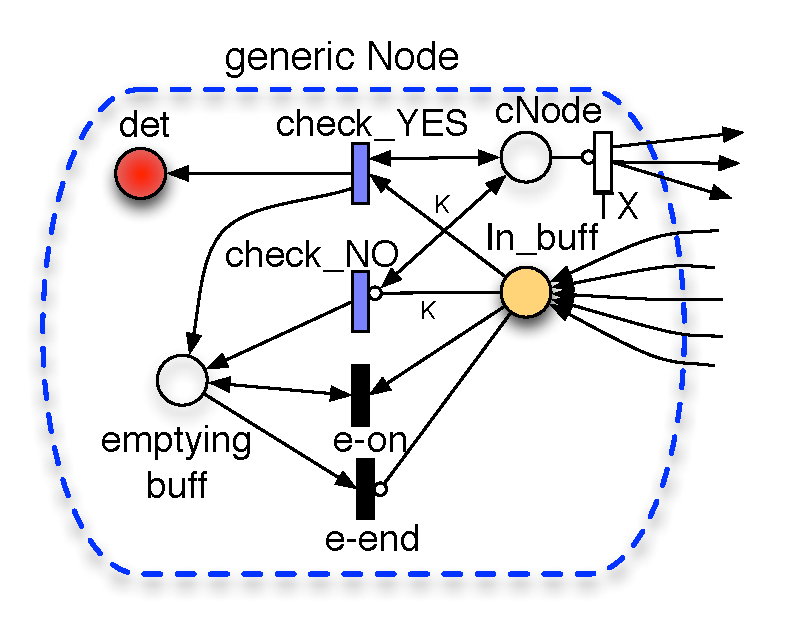
\includegraphics[width=.6\linewidth]{\chapterfig/genNode_GSPN.pdf}
    \caption{Modèle RPSGE d'un \cn élu de manière \emph{dynamique}}\label{sa:fig:cnodegspn2}
\end{figure}

        \subsubsection{Modélisation du cluster}

            \paragraph{\cns élus de façon statique}
Maintenant que la représentation des nœuds individuels a été donnée, nous sommes en mesure de modéliser notre réseau.
Nous travaillons toujours dans un unique cluster.
Pour simplifier la représentation graphique, nous choisissons de représenter un cluster comportant un total de neuf nœuds placés sur une grille de dimensions $3\times3$.
Parmi ces nœuds, deux exactement jouent le rôle de \cn (les nœuds \textsf{3} et \textsf{4} dans notre cas), et un exactement (le nœud \textsf{1}) est un capteur compromis (distinct des \cns).
Cette représentation peut être facilement étendue pour modéliser le réseau tout entier.
La représentation du cluster est donnée en figure~\ref{sa:fig:petricluster}.
\begin{figure}[H]
    \centering
    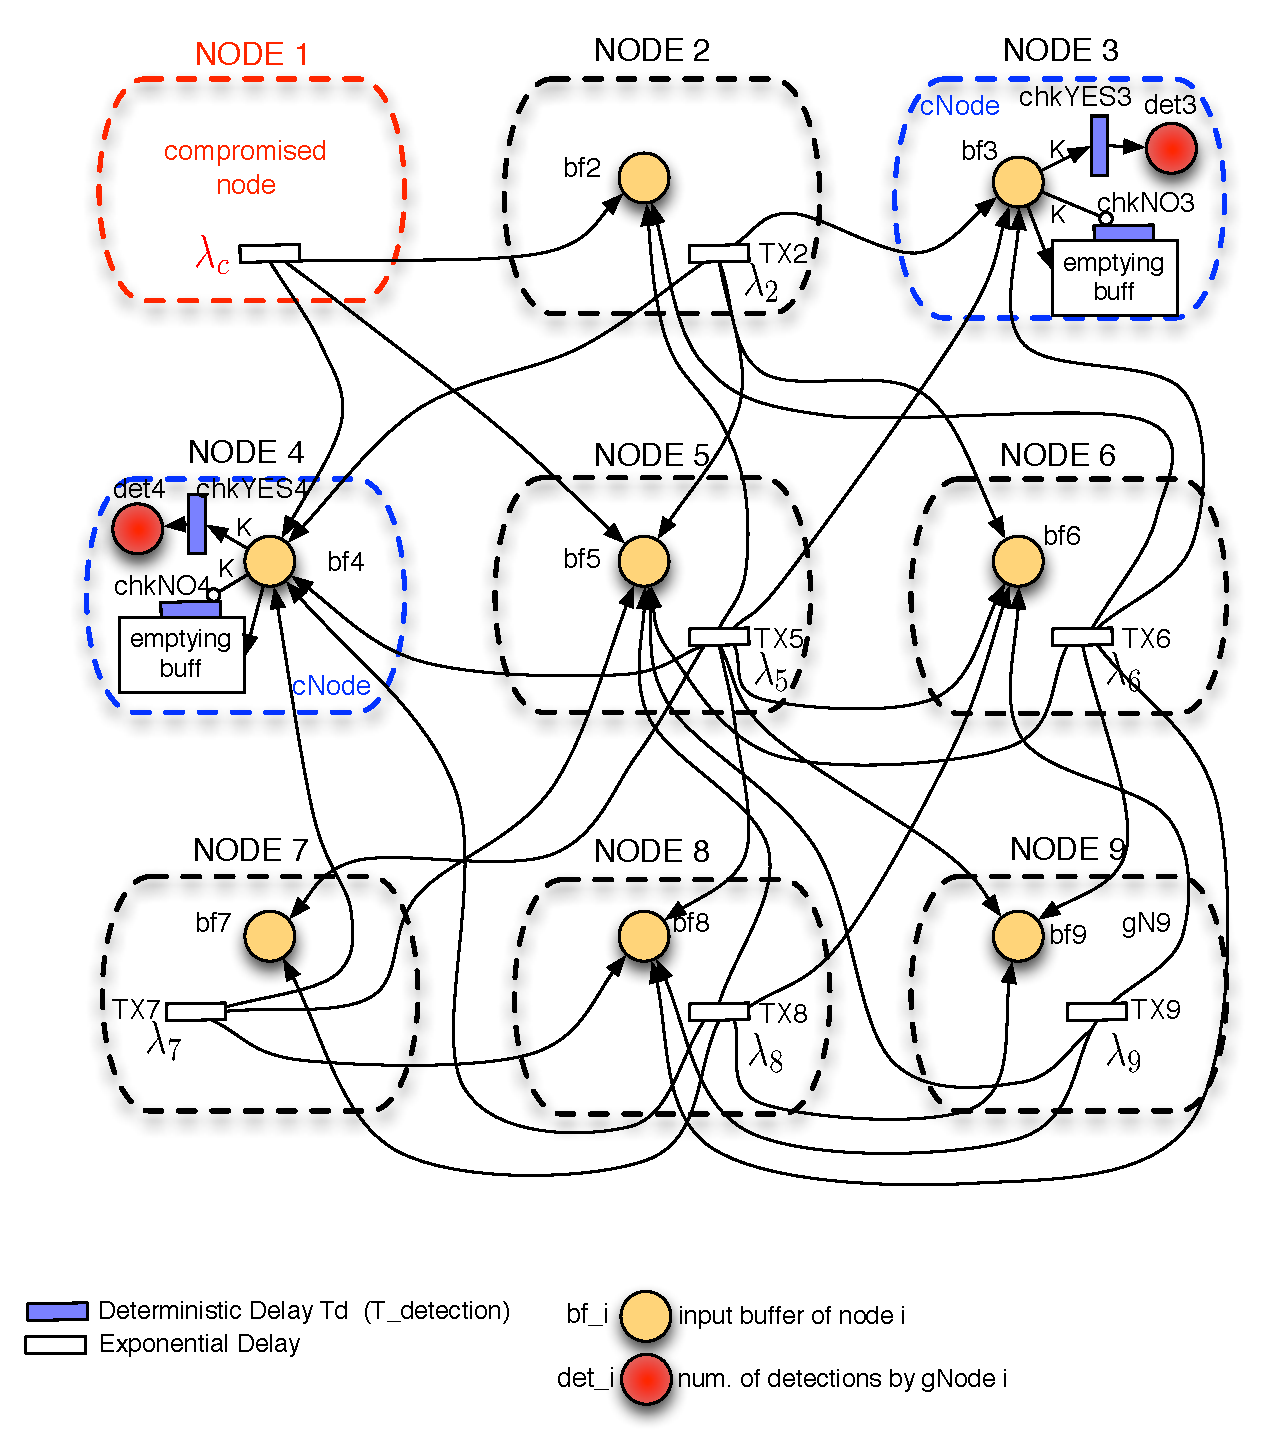
\includegraphics[width=\linewidth]{\chapterfig/PetriNet_DoS_9x9_fixedGnodes.pdf}
    \caption{Modèle RPSGE d'un cluster (topologie: grille $3\times3$) comprenant un nœud compromis et deux \cns statiques}\label{sa:fig:petricluster}
\end{figure}
Également dans l'optique de simplifier la représentation graphique, les transitions \textsf{e-on} et \textsf{e-end}, ainsi que la place \textsf{emptying buff}, ont été remplacées par une boite blanche associée à la fonction de vidage de la place \textsf{In\_buff} des nœuds.

            \paragraph{\cns élus de façon dynamique}
L'élection dynamique des \cns vient compliquer un peu la modélisation de notre cluster.
Bien évidemment, tous les nœuds seront représentés selon le modèle ambivalent illustré par la figure~\ref{sa:fig:cnodegspn2}.
Mais il est aussi nécessaire de rajouter un module qui permettra l'élection des \cns pour chaque période.
Pour une meilleure clarté, le cluster sera représenté en deux temps.
Tout d'abord, la figure~\ref{sa:fig:petridyn} représente le cluster comme nous l'avons vu jusqu'ici, du point de vue du trafic.
\begin{figure}[ht]
    \centering
    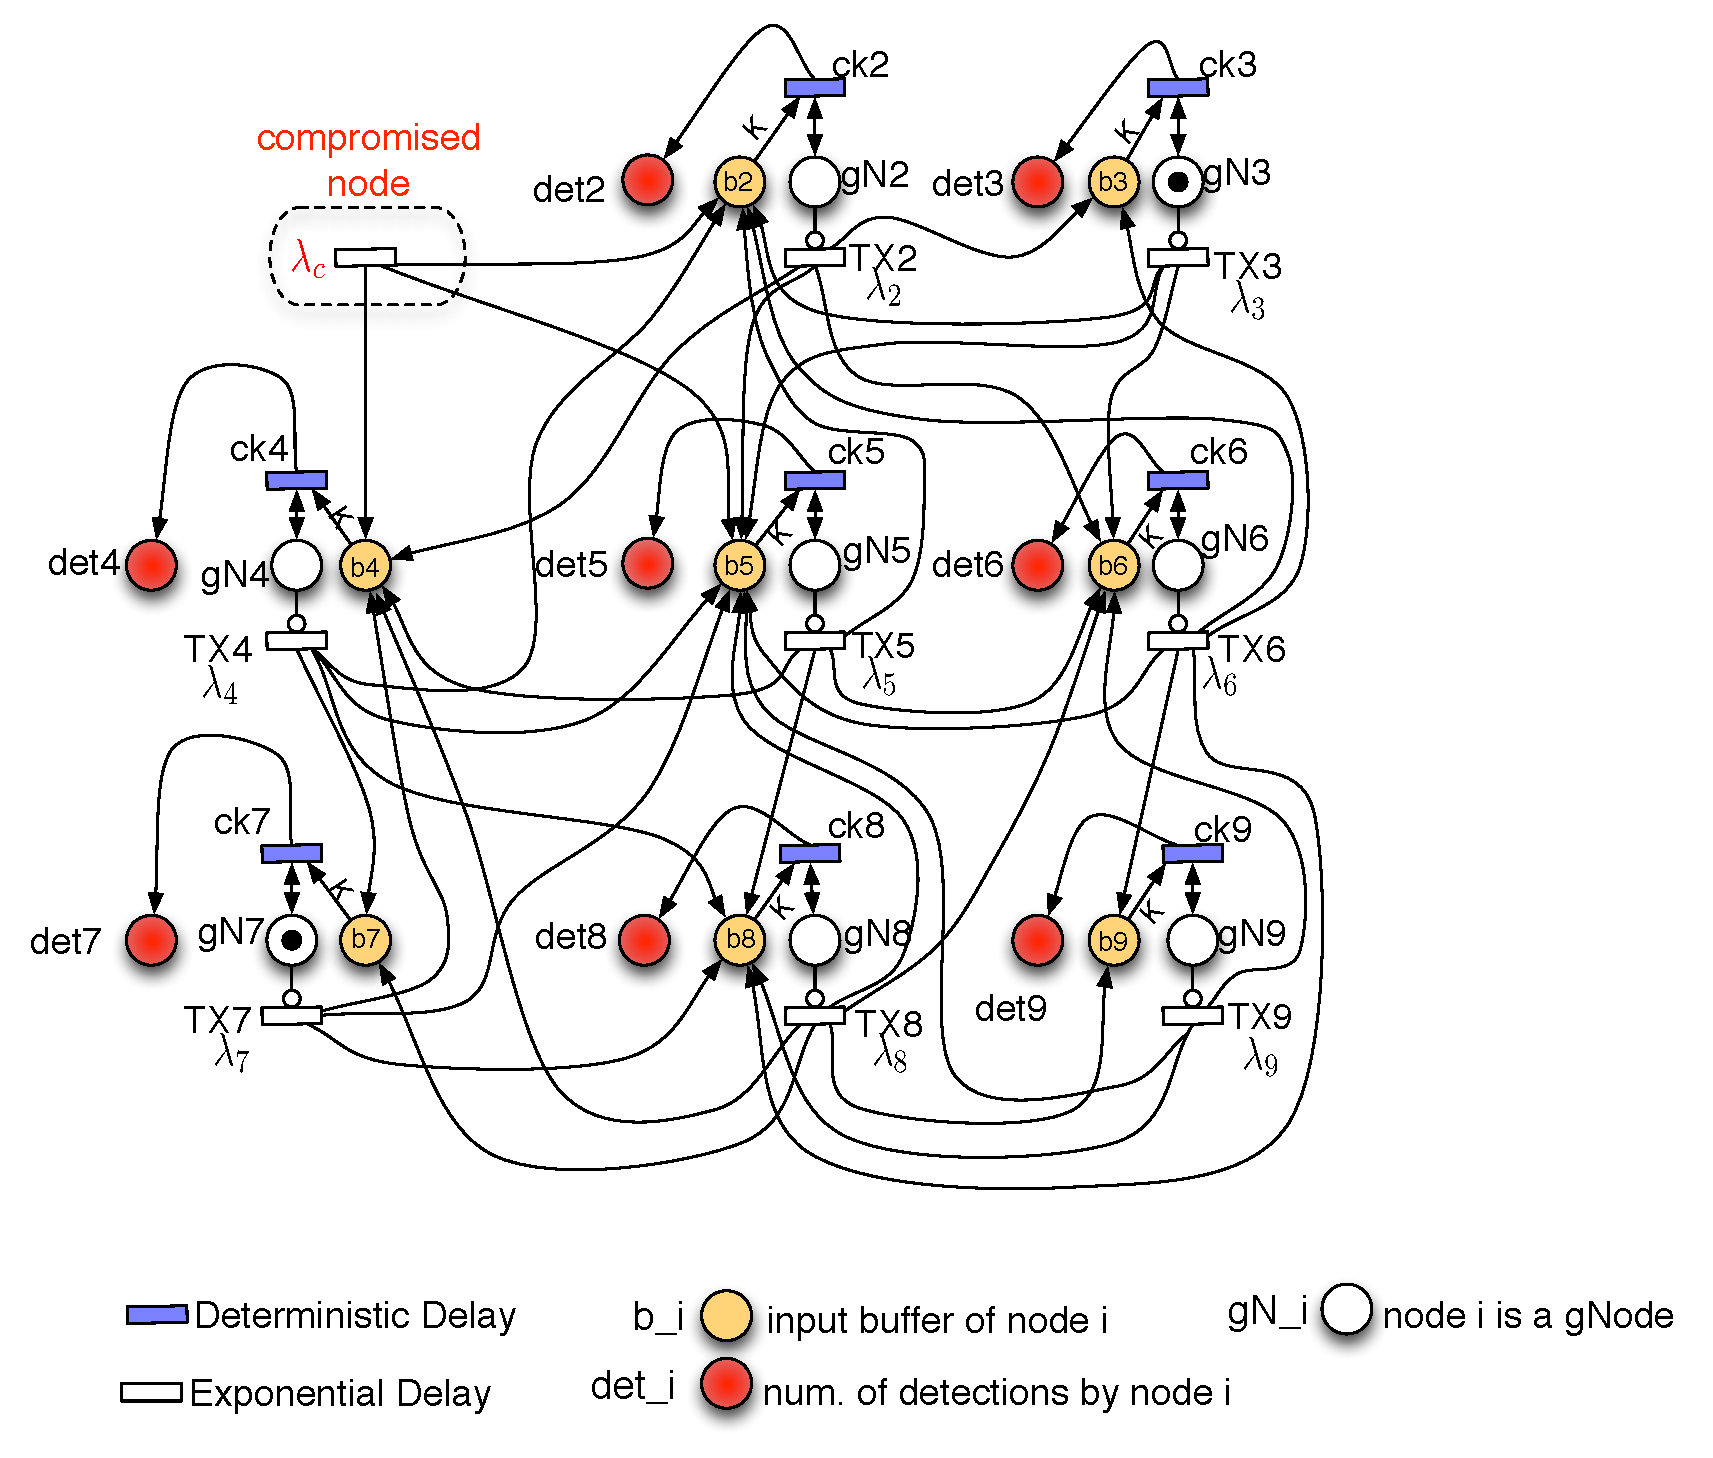
\includegraphics[width=\linewidth]{\chapterfig/PetriNet_DoS_9x9_noElection.pdf}
    \caption{Modèle RPSGE pour le trafic d'un cluster (topologie: grille $3\times3$) comprenant un nœud compromis et deux \cns élus de façon dynamique}\label{sa:fig:petridyn}
\end{figure}
Les huit nœuds non compromis peuvent endosser alternativement les rôles de capteur simple et de \cn (leur représentation a été simplifiée par rapport à la figure~\ref{sa:fig:cnodegspn2}).

\begin{figure}[ht]
    \centering
    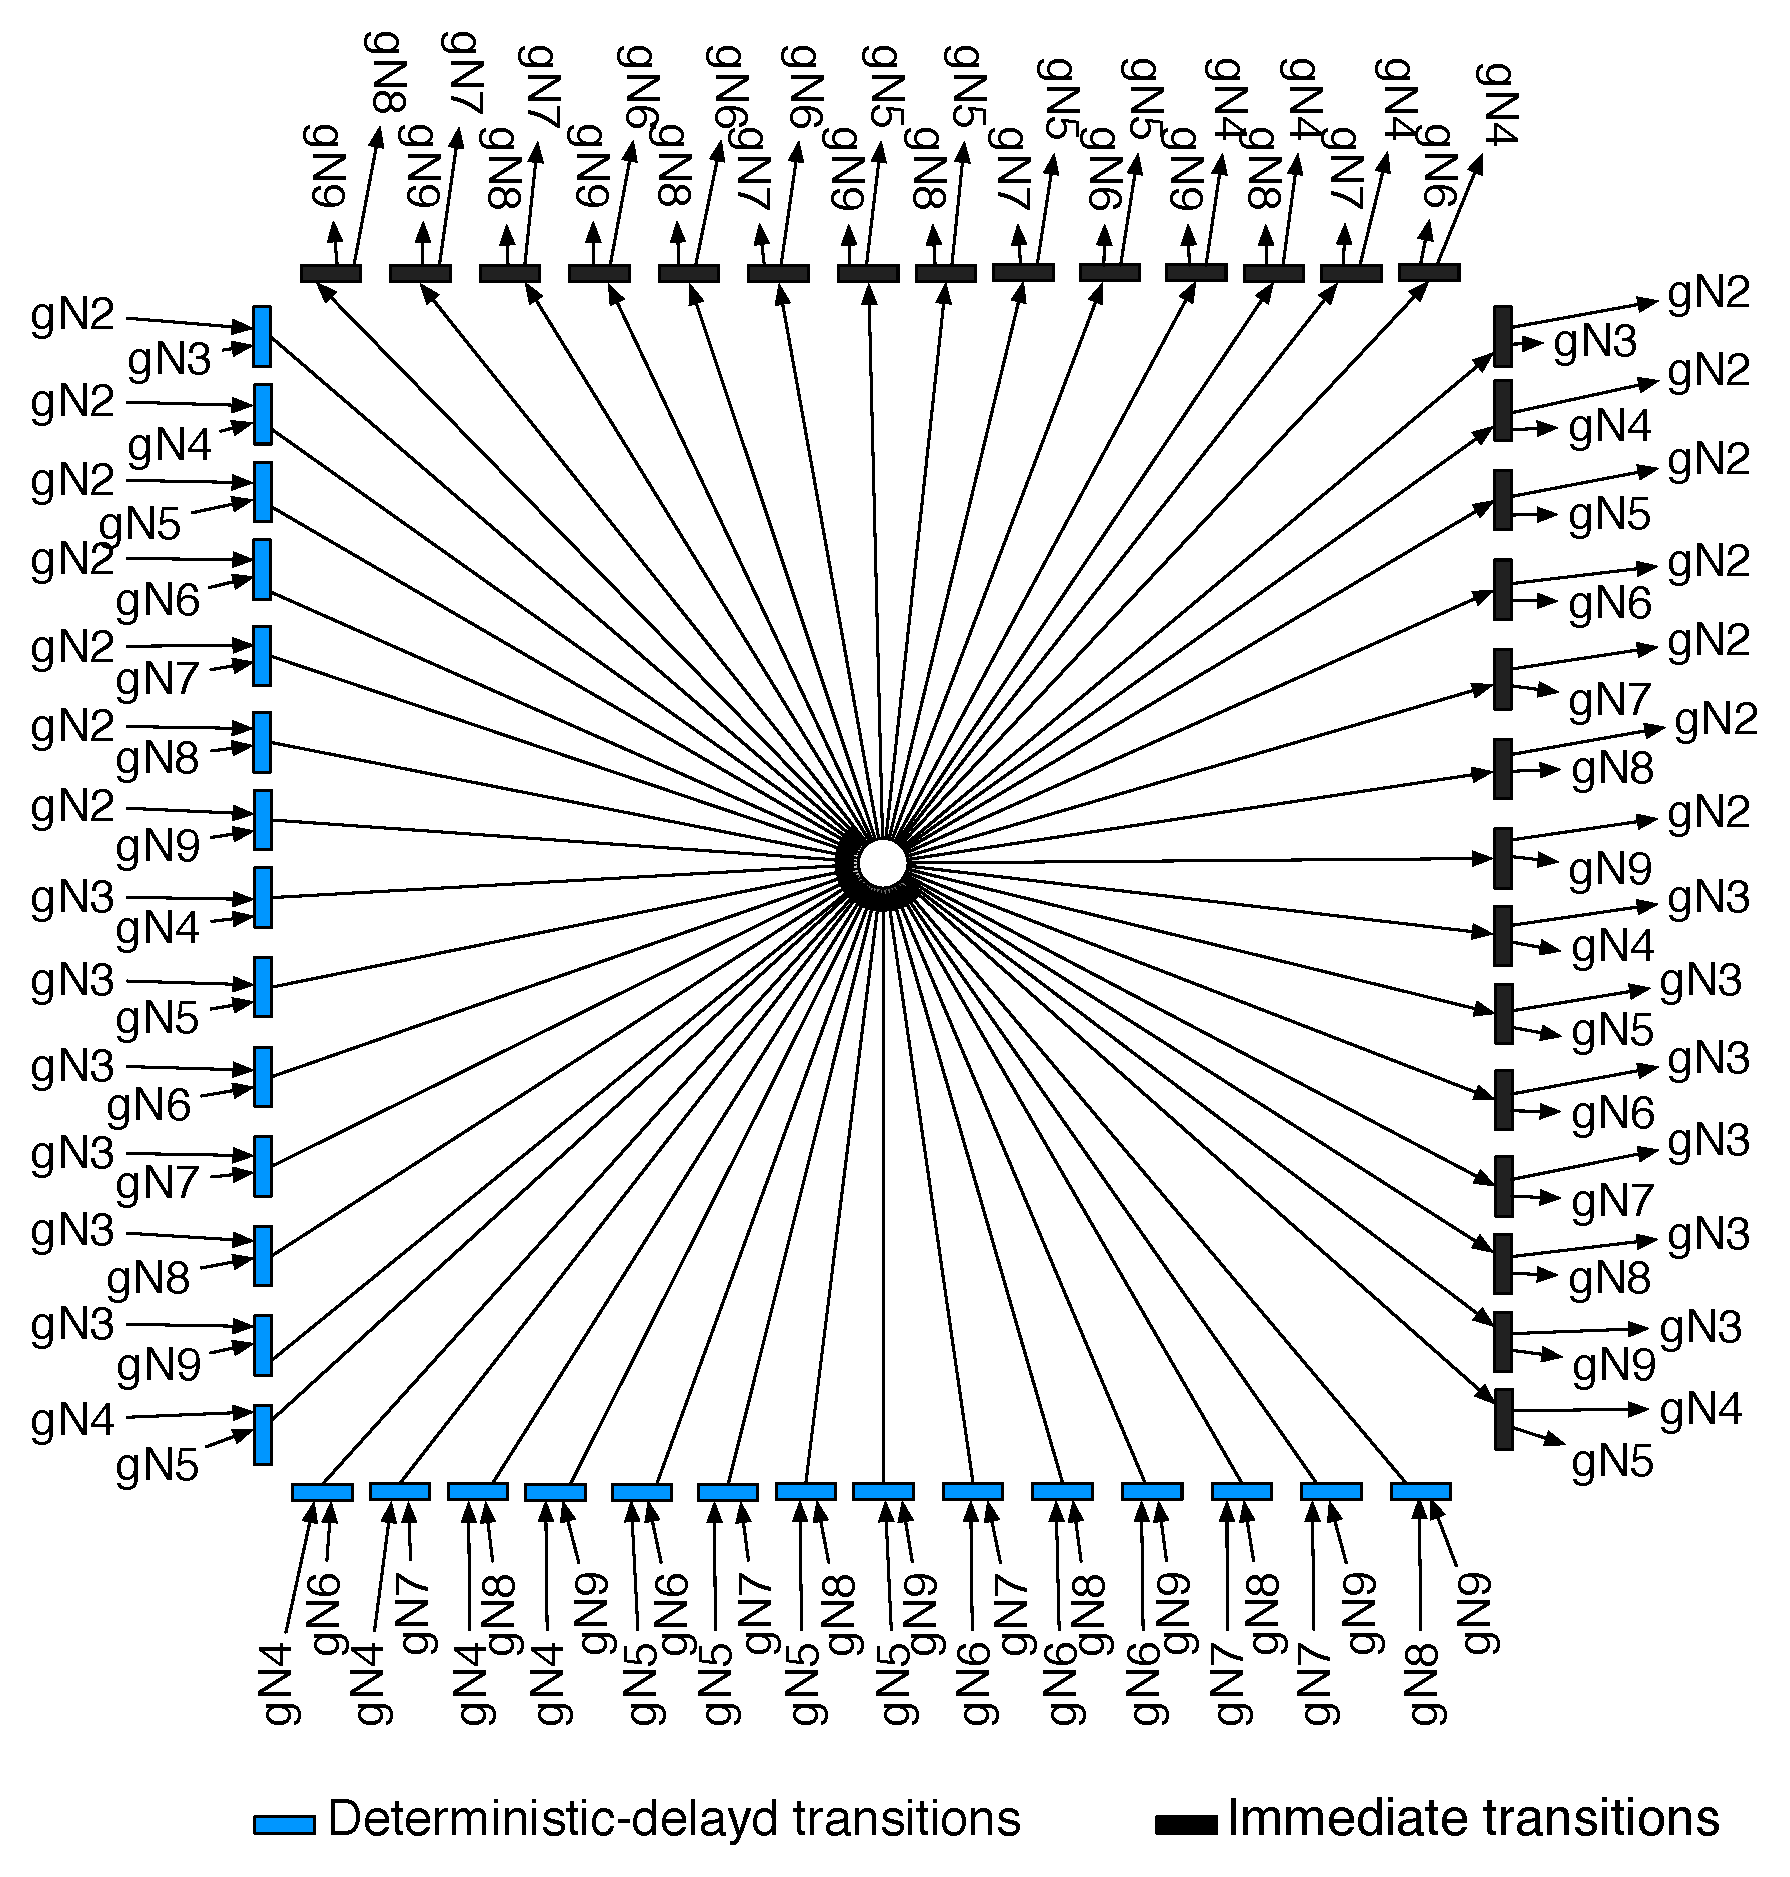
\includegraphics[width=\linewidth]{\chapterfig/PetriNet_DoS_9x9_gNodeElection.pdf}
    \caption{Modèle RPSGE pour l'élection dynamique de deux \cns parmi les nœuds du cluster}\label{sa:fig:petrielec}
\end{figure}
En considérant $n$ comme le nombre de résultats possibles à l'élection, le module représentant l'élection dynamique des \cns comprend:
\begin{itemize}
    \item une unique place centrale;
    \item $n$ transitions minutées, suivant une distribution déterministe, et mutuellement exclusives, menant à cette place (en bleu sur la figure~\ref{sa:fig:petrielec});
    \item $n$ transitions immédiates et mutuellement exclusives, franchissables depuis cette place (en noir sur la figure~\ref{sa:fig:petrielec}).
\end{itemize}
Dans notre cas, pour élire deux \cns au sein du cluster, et en supposant que le nœud compromis ne peut être élu, nous avons $n=\binom{8}{2}=28$~issues possible pour l'élection.
À la fin d'une période d'activité des \cns, une nouvelle élection est déclenchée.
La transition minutée correspondant aux \cns élus pour la période qui s'achève est déclenchée; les jetons présents dans les places \textsf{cNode} de ces \cns sont consommés, et produisent ainsi un jeton dans l'unique place centrale du module.
Chaque transition immédiate tente alors de produire un jeton.
Comme elles sont mutuellement exclusives, mais ont la même priorité et le même poids (voir \sssref{sa:subsubsec:presRPSGE}), un tirage aléatoire a lieu pour déterminer l'unique transition qui est franchie et produit ses jetons.
Ceux-ci sont envoyés dans les places \textsf{cNode} des nœuds élus pour la période qui débute, activant au passage leurs fonctionnalités de \cns.
%===============================================================================
    \subsection{Logique stochastique avec automates hybrides}

        \subsubsection{Présentation de la logique stochastique avec automates hybrides}
La logique stochastique avec automates hybrides (LSAH, ou bien \textit{Hybrid Automata Stochastic Logic}, \textit{HASL}) est un langage récent, qui introduit un framework regroupant des études de \textit{model checking} et d'évaluation des performances ainsi que de fiabilité sur des processus stochastiques à événements discrets (PSED) exprimés sous forme de réseaux de Petri sthochastiques généralisés (RPSG)~\cite{BDDHP11hasl}.
Plus concrètement, à partir d'un modèle RPSG, les mesures de performances sont exprimées à l'aide de formules LSAH avant que leur soit appliquées des fonctions de \textit{model checking} statique permettant de vérifier automatiquement ces formules.
%en place de vérifications, en termes d'études statistiques, de modèles stochastiques~\cite{BDDHP11hasl}.

Pour bien comprendre le fonctionnement de LSAH, voici quelques rappels sur le \textit{model checking}: il s'agit d'une procédure de vérification formelle utilisant:
\begin{itemize}
    \item un modèle $M$ à états discrets;
    \item une propriété formelle exprimée par une formule de logique temporelle $\phi$.
\end{itemize}
Un algorithme est alors utilisé pour déterminer automatiquement si $\phi$ vérifie $M$ (ce que l'on note $M\models\phi$).
Dans le cas d'un modèle stochastique, des probabilités sont associées aux formules.
Vérifier que $M\models\phi$ revient alors à déterminer la probabilité de la formule $\phi$ dans le contexte du modèle $M$.
LSAH étend ce concept dans le sens où l'évaluation d'une formule peut donner n'importe quel nombre réel, et représenter ainsi une probabilité aussi bien que toute autre mesure de performance.
À cette fin, LSAH fait appel à des automates linéaires hybrides (ALH).
Un ALH résulte, de manière résumée, de la généralisation des automates temporels dont les variables «~horloges~» sont remplacées par des variables de données réellement évaluées.
Basée sur ce modèle une formule LSAH comprend ainsi deux sous-éléments:
\begin{itemize}
    \item un ALH permettant la sélection des exécutions temporelles à retenir à partir du modèle RPSG considéré, cette sélection étant le fruit de la syncronisation entre une exécution générée par le modèle RPSG et l'ALH;
    \item une expression $Z$, représentant la mesure à évaluer, construite à l'aide des variables de l'ALH selon la syntaxe suivante:
    \[
        \begin{split}
            Z ::= & \ E(Y)\ |\ Z+Z\ |\ Z \times Z\\
            Y ::= & \ c\ |\ Y+Y\ |\ Y \times Y\ |\ Y/Y\ |\ \mbox{last}(y)\ |\ \mbox{min}(y)\\
                  & \ \  |\ \mbox{max}(y)\ |\ \mbox{int}(y)\ |\ \mbox{avg}(y)\\
            y ::= & \ c\ |\ x\ |\ y+y\ |\ y \times y\ |\ y/y
        \end{split}
    \]
    Cette expression peut être interprétée comme suit:
    \begin{itemize}
        \item $x$ est une variable de données de l'automate:
        \item $y$ est une expression arithmétique à partir de ces variables de données;
        \item $Y$ est une variable de chemin aléatoire, \cad une variable évaluée à l'aide d'un chemin de syncronisation, lui-même créé par la syncronisation entre une trajectoire du modèle RPSG et l'ALH;
        \item $\mbox{last}(y)$ est la dernière des valeurs endossées par l'expression $y$ le long d'un chemin syncronisé; $\mbox{min}(y)$ et $\mbox{max}(y)$ sont les valeurs optimales obtenues le long de ce chemin. $\mbox{int}(y)$ est l'intégrale d'$y$, et $\mbox{avg}(y)$ la moyenne des valeurs obtenues le long du chemin.
    \end{itemize}
\end{itemize}

Au final, LSAH fonctionne de la façon suivante:
\begin{enumerate}
    \item le système est exprimé sous la forme d'un modèle RPSG et d'une formule LSAH;
    \item LSAH génère de façon itérative les trajectoires à partir de l'espace d'états du modèle RPSG et les syncronise avec l'ALH;
    \item les trajectoires acceptées par l'ALH sont évaluées pour obtenir l'estimation de la mesure étudiée. Les trajectoires refusées sont abandonnées.
\end{enumerate}

        \subsubsection{Automate linéaire hybride et formule LSAH associés au modèle utilisé}
Nous présentons ici quelques exemples de formules LSAH, constitués des expressions LSAH et d'un automate hybride linéaire hybride (ALH) associé au modèle RPSGE présenté plus haut (en figure~\ref{sa:fig:petridyn}).
Ces exemples présentent une manière de mesurer des données sur un nœud du réseau de capteurs à partir de la version modélisée sous forme de réseaux de Petri, à fin d'étude, ou bien de comparaison de notre solution avec d'autres systèmes de détection des attaques de type «~déni de service~».
Ces exemples peuvent en outre être modélisés facilement avec l'outil de \textit{model checking} \textsf{COSMOS}~\cite{BDDHP11cosmos}.

On considère un nœud quelconque $i$ ($1\leq i\leq$~nombre de capteurs).
L'automate linéaire hybride que nous utilisons fait appel aux variables valuées suivantes:
\begin{itemize}
    \item $x_t$: temps global;
    \item $x_{d_i}$: nombre d'attaques détectées par le \cn $i$;
    \item $x_{\mathit{TX}_i}$: nombre de paquets envoyés par le nœud $i$;
    \item $x_{\mathit{bf}_i}$: nombre de paquets reçus et placés dans le tampon en entrée du nœud $i$.
\end{itemize}
L'automate linéaire hybride est présenté en figure~\ref{sa:fig:lha}.
\begin{figure}[H]
    \centering
    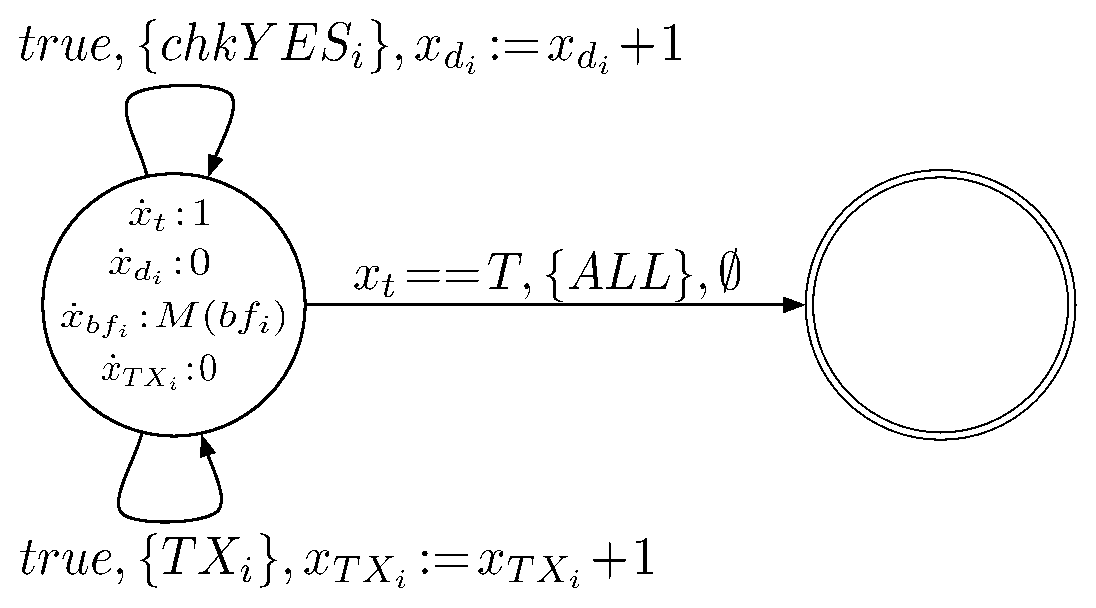
\includegraphics[width=.8\linewidth]{\chapterfig/LHA1.pdf}
    \caption{Automate linéaire hybride permettant d'effectuer des mesures sur le modèle RPSGE proposé}\label{sa:fig:lha}
\end{figure}
Cet automate comprend deux états, et fait références aux variables que nous venons de définir.
Ses transitions sont franchies lorsqu'un élément survient (par exemple: égalité de $x_t$ à $T$, ou franchissement d'une transition sur le modèle RPSGE); nous y reviendrons.
L'état de gauche, que l'on nommera $e_1$, contient le taux de variation (autrement dit, la dérivée première) de chacune des quatre variables décrites:
\begin{itemize}
    \item À chaque unité de temps passée, le temps global (la variable $x_t$) est incrémenté de $\dot{x}_t=1$;
    \item $x_{d_i}$ et $x_{\mathit{TX}_i}$ sont inchangées tant qu'aucune transition du modèle RPSGE n'est franchie.
        Leurs taux de variation $\dot{x}_{d_i}$ et $\dot{x}_{\mathit{TX}_i}$ sont nuls;
    \item $x_{\mathit{bf}_i}$ est incrémentée avec un taux proportionnel au nombre de jetons présents dans le tampon d'entrée de $i$ (lorsque $i$ joue le rôle de \cn).
        On notera ce taux $\dot{x}_{\mathit{bf}_i}$.
\end{itemize}
$e_1$ comporte également trois transitions, exprimées sous la forme suivante: $<$\textit{condition temporelle (sur x\_t)}$>, <$\textit{ensemble des transitions franchies sur le réseau de Petri pour déclencher l'évènement}$>, <$\textit{action associée sur les variables de l'automate}$>$.
Il s'agit des transitions suivantes:
\begin{itemize}
    \item la première transition qui boucle sur $e_1$: $e_1\xrightarrow{\mathit{true},\{\mathsf{chkYES_i}\},(x_{d_i}:=x_{d_i}+1)}{e_1}$.
        Elle correspond à l'évènement associé au passage de la transition \textsf{check\_YES} du nœud $i$ sur le modèle RPSGE du cluster (présenté en figure~\ref{sa:fig:petridyn}).
        Lorsque la transition est franchie sur le réseau de Petri, quelle que soit la valeur de l'«~horloge~» $x_t$ (condition $\mathit{true}$), la transition correspondante sur l'automate linéaire hybride est elle-aussi franchie\footnote{Attention: les transitions du réseau de Petri, représentées par des rectangles et reliées aux places par des arcs, ne doivent pas être confondues avec les transitions des automates, représentées par des arcs, et reliant les états.}.
        Comme la transition du réseau de Petri correspond à une nouvelle détection de trafic anormal par le nœud $i$, la transition de l'automate a pour effet de mettre à jour la valeur de $x_{d_i}$, en l'incrémentant de $1$;
    \item une deuxième transition qui boucle elle aussi sur $e_1$: $e_1\xrightarrow{\mathit{true},\{\mathsf{TX_i}\},(x_{\mathit{TX}_i}:=x_{\mathit{TX}_i}+1)}{e_1}$.
        Cette transition fonctionne de façon identique à la précédente, à la différence près que la transition du réseau de Petri concernée n'est plus \textsf{check\_YES} mais \textsf{TX}, et la variable de l'automate est $x_{\mathit{TX}_i}$: lorsque le nœud $i$ envoie un message (et que \textsf{TX} est franchie sur le modèle RPSGE), la variable $x_{\mathit{TX}_i}$ est incrémentée de $1$;
    \item une dernière transition qui mène de $e_1$ à $e_2$.
        Cette transition conduit à l'état final de l'automate, qui accepte et valide le chemin des transitions parcourues pour l'étudier à l'aide des formules LSAH: $e_1\xrightarrow{(x_t==T),\{\mathit{ALL}\},\emptyset}{e_2}$.
        La transition est autorisée lorsque $x_t$ vaut $T$, autrement dit: elle est déclenchée toutes les $T$ unités de temps.
        Elle accepte donc n'importe quel chemin dans l'automate, dont la durée est de $T$ unités de temps.
        Elle ne dépend pas d'une transition particulière du modèle RPSGE (puisqu'elle les acceptes toutes, $\{\mathit{ALL}\}$).
        Aucune action sur les variables n'est effectuée lorsque la transition est franchie.
\end{itemize}

Une fois un chemin validé par l'automate, il peut être analysé à l'aide de formule LSAH.
Voici quelques exemples de formules LSAH permettant d'obtenir plusieurs valeurs sur le cluster considéré à partir des variables définies plus haut pour l'automate:
\begin{itemize}
    \item $Z_1\equiv E(\mbox{last}(x_{d_i}))$: le nombre attendu d'attaques détectées par le \cn $i$ après $T$ unités de temps;
    \item $Z_2\equiv E(\mbox{last}(x_{d_i}+x_{d_{i'}}))$: la somme attendue des attaques détectées par les nœuds $i$ et $i'$ après $T$ unités de temps;
    \item $Z_3\equiv E(\mbox{last}(x_{\mathit{TX}_i}))$: le nombre attendu de paquets envoyés par le nœud $i$ après $T$ unités de temps;
    \item $Z_4\equiv E(\mbox{int}(x_{\mathit{bf}_i}))$: le cumul attendu du nombre de paquets reçus par le nœud $i$ après $T$ unités de temps.
\end{itemize}

%===============================================================================
    \subsection{Conclusion}

Ici se termine la section sur la modélisation.
Après avoir étudié les limites des processus markoviens, qui sont orientés vers la modélisation d'événements à distribution exponentielle, nous avons présenté deux autres évaluations formelles possibles pour notre solution.
L'une d'elles a fait intervenir une version étendue des réseaux de Petri, dédiée à la représentation de toutes sortes de distributions événementielles, et permet la visualisation de la solution sous l'aspect classique des réseaux de Petri.
La dernière est basée sur un langage récent, la logique stochastique avec automates hybrides, et permet l'évaluation formelle des performances de notre solution.
Toutes ont bien sûr pour objectif de modéliser notre solution afin d'en souligner les avantages et inconvénients, mais aussi de présenter aux lecteurs différents moyens existants d'employer les méthodes formelles en vue de modéliser des réseaux de capteurs, et ce de façon plus générale que dans le seul contexte de notre solution.

Évidemment, malgré tous ses attraits la modélisation ne peut se substituer à une évaluation numérique de la solution, comme nous allons le présenter, dans la section suivante, par le biais des résultats obtenus à l'aide d'une simulation.


% vim: set spelllang=fr foldmethod=marker:
\section{Simulation du processus}\label{se:sec:simul}

    \subsection{Résultats numériques}
Le processus de sélection des \cns selon leur énergie résiduelle a, lui aussi, conduit à la réalisation de plusieurs simulations, afin de le comparer au modèle de sélection pseudo-aléatoire.
Le logiciel \nsiii~\cite{ns3} a été utilisé pour l'occasion.

Plusieurs instances de simulation ont été réalisées, avec l'accent porté sur les valeurs de l'énergie consommée ainsi que sur la répartition de la charge dans le cluster.
Les mécanismes de détection des deux méthodes sont quasiment identiques, et fournissent donc des résultats similaires à ceux obtenus au chapitre précédent en \ssref{sa:ssec:detec} (sur la méthode avec renouvellement périodique) pour ce qui est du taux de détection des nœuds compromis.
Les paramètres utilisés lors des simulations sont présentés en \tabref{se:table:parameters}.

\begin{table}[!ht]
    \centering
    \caption{Paramètres de simulation}
    \medskip
    \begin{tabular}{l l}
        \toprule
        \textsc{Paramètre}                 & \textsc{Valeur}\\
        \midrule
        Nombre de nœuds                    & 30 (plus 1~\CH)\\
        Nombre de \cns                     & 4\\
        Probabilité de sélection d'un \vns & 33~\%\\
        Période de renouvellement des \cns & 1~minute\\
        Durée totale de simulation         & 30~minutes\\
        Forme du cluster                   & carré\\
        Taille du cluster                  & 2$\times$50~mètres de diagonale\\
        Portée de transmission             & 50~mètres\\
        Position des nœuds                 & \CH: au centre; autres: aléatoire\\
        Mobilité des nœuds                 & nulle\\
        Débit d'émission des nœuds normaux & 1024~octets toutes les 3~secondes\\
        Requêtes des \vns (par \cn cible)  & 1024~octets toutes les 5~secondes\\
        \bottomrule
    \end{tabular}\label{se:table:parameters}
\end{table}

Ces simulations ont permis d'obtenir l'énergie résiduelle de chaque capteur à intervalles réguliers (une fois par minute).
À partir de ces données, nous avons pu retracer les courbes d'évolution de la moyenne et de l'écart-type de la distribution de l'énergie résiduelle entre les nœuds.
L'énergie résiduelle du \ch a été volontairement ignorée.
\begin{figure}[!b]
    \centering
    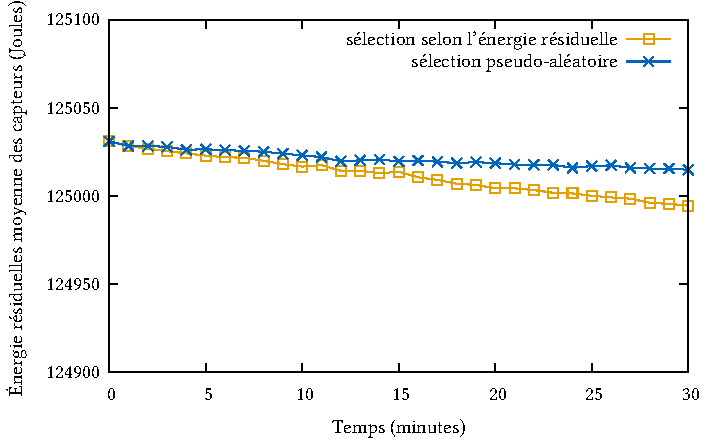
\includegraphics[width=.96\linewidth]{\chapterfig/plot_se_mean.pdf}
    \caption[Valeur moyenne de l'énergie des nœuds en fonction du temps]{Valeur moyenne de l'énergie des nœuds (à l'exception du \ch) en fonction du temps}\label{se:fig:mean}
\end{figure}
La valeur moyenne est présentée sur la \figref{se:fig:mean}.
L'augmentation des valeurs à $t=11$~minutes ainsi qu'à $t=15$~minutes sur la courbe de la sélection par l'énergie provient de l'effet de récupération des batteries.
Ces résultats sont conformes aux attentes: le processus de sélection par l'énergie consomme davantage d'énergie dans le réseau, ce que l'on peut imputer au rôle supplémentaire de \vn mis en place.
Étant donné que les \vns vont avoir à sortir périodiquement de leur état de veille pour envoyer une requête au \cn surveillé, écouter la réponse, et calculer une consommation théorique, le besoin en ressources énergétiques se retrouve logiquement affecté par rapport au processus de sélection pseudo-aléatoire.

Le volume de données de contrôle pour les deux méthodes proposées apparait sur la \figref{se:fig:overhead}.
Ici encore, l'usage des \vns entraine une augmentation des ressources consommées; il faut également tenir compte des messages (moins nombreux) envoyés par chaque capteur au moment du renouvellement de la sélection.
\begin{figure}[!ht]
    \centering
    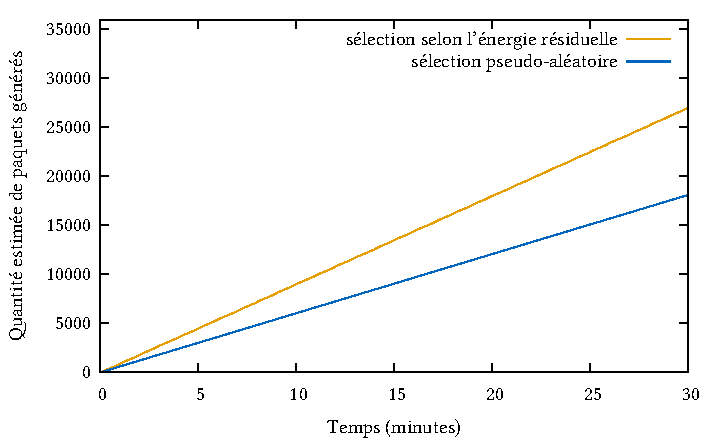
\includegraphics[width=.96\linewidth]{\chapterfig/plot_se_overhead.pdf}
    \caption{Estimation du nombre total de paquets générés au cours de la simulation au cours du temps}\label{se:fig:overhead}
\end{figure}

L'écart-type de la distribution en énergie résiduelle des nœuds est présenté sur la \figref{se:fig:stddev}.
Durant les premières minutes de la simulation, la sélection par l'énergie crée une dispersion plus affirmée de la charge en énergie du réseau, à cause des \vns (il y a davantage de capteurs qui endossent des rôles consommant plus d'énergie).
Mais après les sept premières minutes environ, l'écart-type pour le processus de sélection par l'énergie devient et demeure inférieur à celui associé à la méthode pseudo-aléatoire.
Cela traduit la meilleure répartition de la charge énergétique dans le cluster, ce qui était l'objectif initial de la solution proposée dans ce chapitre.
La différence entre les écart-types des deux méthodes est malgré tout peu élevée: cela tient entre autres aux modèles implémentés pour les simulations.
Comme nous disposons d'un générateur de nombres pseudo-aléatoires efficace, à partir d'un certain nombre de renouvellements de la sélection, tous les capteurs vont endosser le rôle de \cn à peu près le même nombre de fois si la sélection se fait de façon pseudo-aléatoire.
Et comme les capteurs ont également des activités de mesure identique, cette méthode (pseudo-aléatoire) fournit, dans notre cas, une excellente répartition de la charge dans le cluster.
Dans une situation où les capteurs auraient des niveaux d'activité différents ---~si par exemple un évènement à détecter se produit beaucoup plus souvent dans une certaine région géographique du cluster~--- alors la consommation, avec cette méthode, ne serait plus nécessairement équilibrée entre tous les nœuds du cluster.
Tandis que la sélection des \cns par l'énergie résiduelle permettrait de rétablir cet équilibre.
\begin{figure}[!ht]
    \centering
    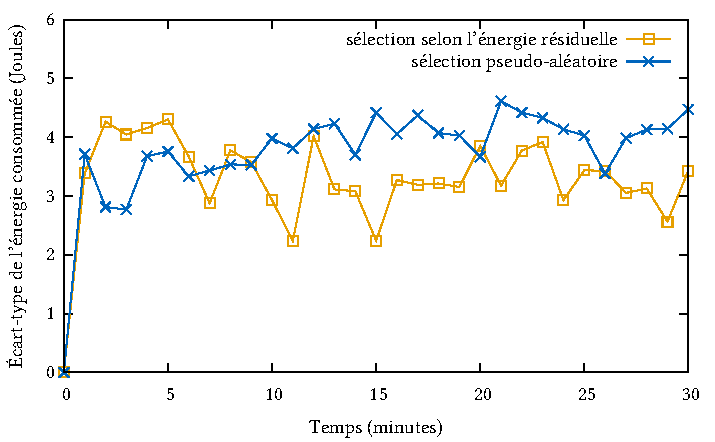
\includegraphics[width=.96\linewidth]{\chapterfig/plot_se_stddev.pdf}
    \caption[Écart-type pour l'énergie résiduelle des nœuds au cours du temps]{Écart-type pour l'énergie résiduelle des nœuds (à l'exception du \ch) au cours du temps}\label{se:fig:stddev}
\end{figure}

    \subsection{Pousser plus loin l'amélioration}

Par rapport au processus d'auto-désignation pseudo-aléatoire introduit dans le chapitre précédent, le second mécanisme proposé prend en compte l'énergie résiduelle de chaque nœud au moment de renouveler les \cns, ce qui assure une meilleure répartition de la consommation en énergie dans le cluster.
Mais si elle est mieux répartie, l'énergie consommée l'est aussi en plus grande quantité, principalement à cause de l'usage nouveau des \vns.
Les requêtes et les réponses aux \cns consomment de l'énergie, et viennent alourdir l'implémentation de la solution: il y a trois rôles différents assignés dans le cluster (sans compter le \ch), et deux d'entre eux nécessitent une étape spécifique pour leur attribution.

Il serait commode de pouvoir se passer des \vns, mais sans faire de concessions sur la sécurité.
L'idéal serait de pouvoir réutiliser les observations des \cns antérieurs pour mettre en place un mécanisme de sélection qui tienne compte de l'énergie résiduelle, voire même d'un ensemble de paramètres permettant de choisir les meilleurs candidats.
Ce jeu de paramètres, s'il inclue un score de confiance, peut même venir renforcer la sécurité du dispositif.
C'est sur cet axe que s'appuient les améliorations proposées dans le prochain chapitre.

